\documentclass{article}

\usepackage[utf8]{inputenc}
\usepackage[left=1in,right=1in,bottom=1in]{geometry}
\setlength\parindent{0pt}
\setlength{\parskip}{1em}
\setcounter{secnumdepth}{0}
\usepackage{outlines}
\usepackage{hyperref}
\usepackage{graphicx}
\graphicspath{ {imgs} }
\usepackage{color,soul}

\title{Urban Social Geography}
\author{Carla Hyenne }

\begin{document}

\maketitle

\tableofcontents

%%%%%%%%%%%%%%%%%%%%%%%%%%%%%%%%%%%%%%%%%%%%%%%%%%%%
%																LECTURE 1
%%%%%%%%%%%%%%%%%%%%%%%%%%%%%%%%%%%%%%%%%%%%%%%%%%%%

\pagebreak\section{Urban Geographical Traditions}
\textit{September 27th, 2021}

\textit{tldr; draw a general outline of how urban geography has been practiced in the last 50 years, and how it interrogates some of urban geography's main concepts and approaches.}

\subsection{What is ``the urban''?}

\subsubsection{Urban Age}

We are living in the Urban Age, where the population growth is proportional to urban growth. Since circa 2005, the majority (more than 50\%) lives in urban areas, or cities, as opposed to rural areas.

Urbanization is a \textbf{global phenomenon}. It started with the global North (USA, Western Europe) in the 19th century, spread to South America, USSR, Oceania in the 1950s, and Africa, Asia in the 1990s. Urbanisation intensified in the 1990s, and as of the 2000s, Asia dominates the economic growth and urbanisation.

Urbanization isn't equal throughout the world. For example, in 2018, ~40\% of Africa's population was urban, ~50\% in Asia, ~75\% in Europe, ~80\% in Latin America and North America, and ~70\% in Oceania.

\begin{center}
	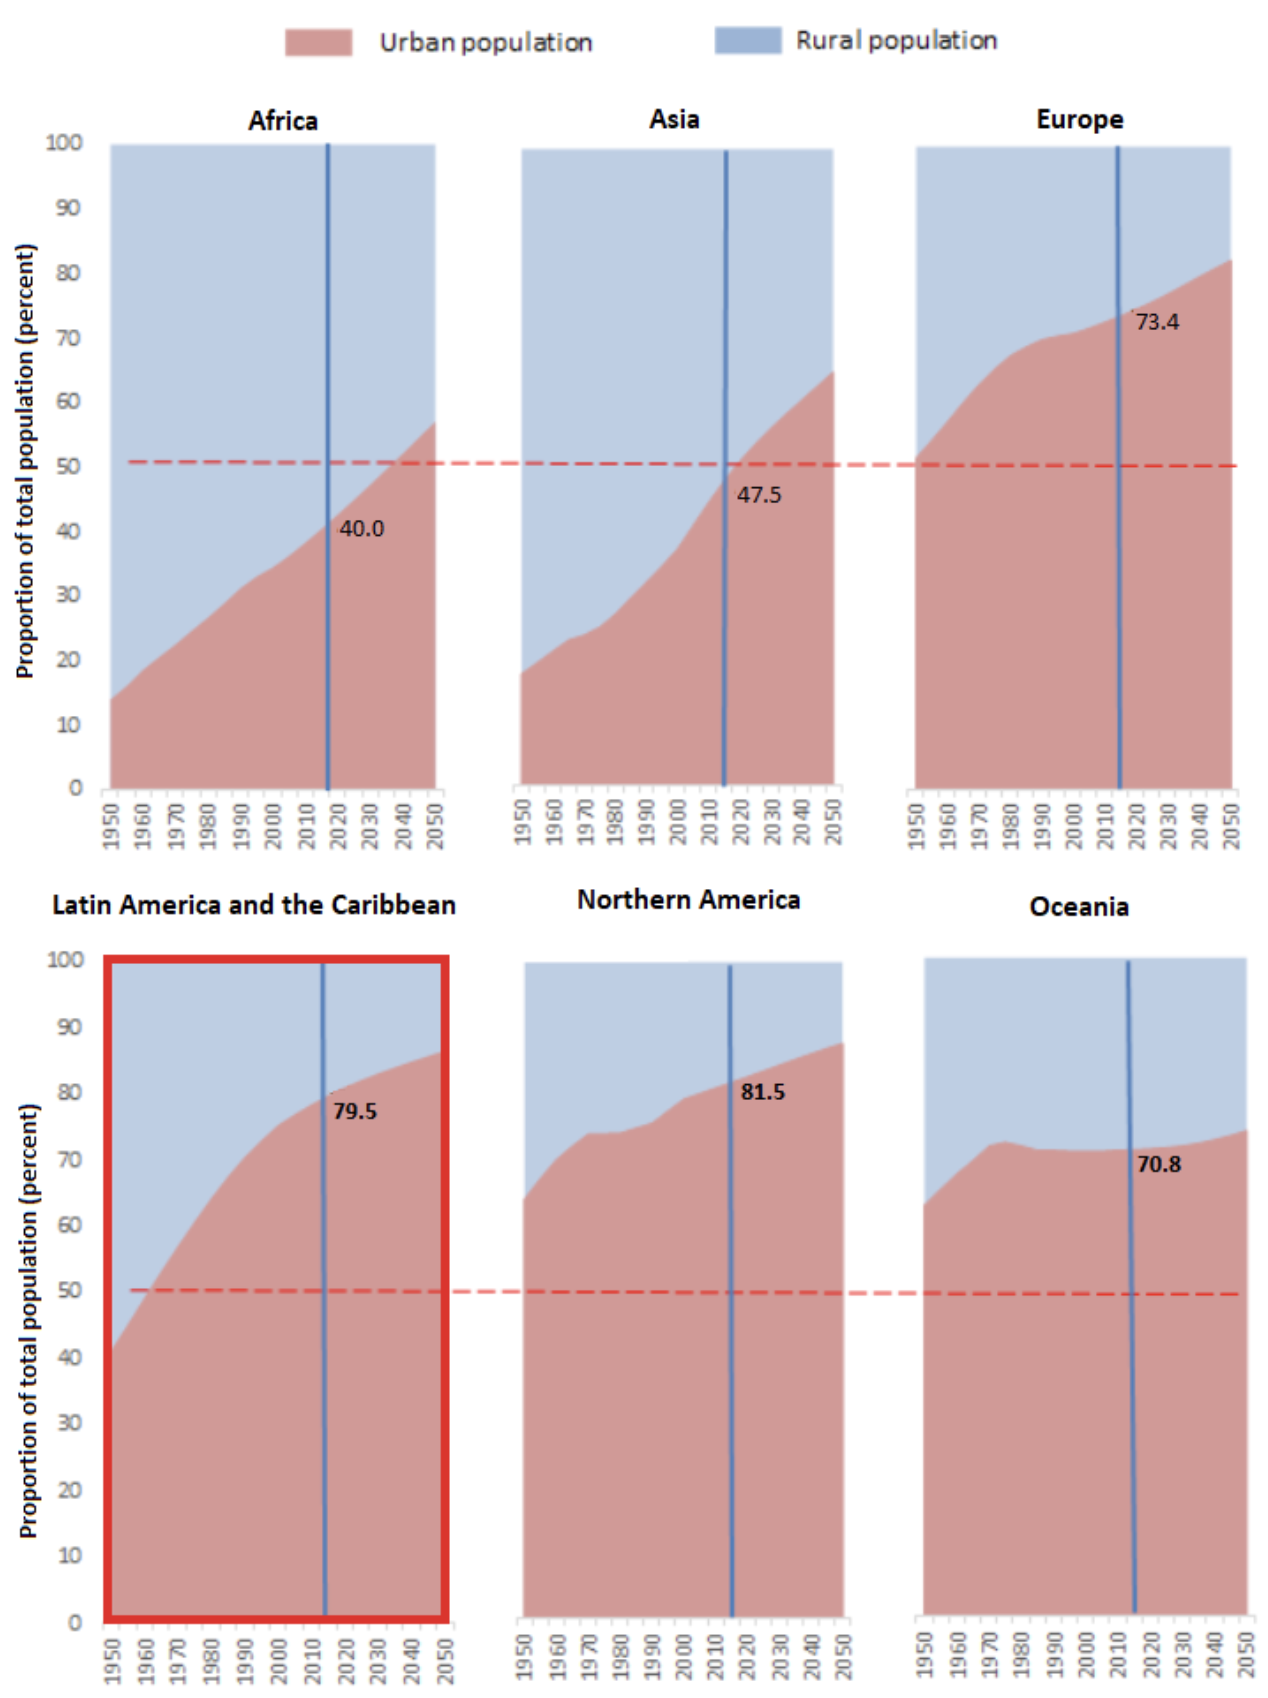
\includegraphics[width=30em]{urban_rural_proportion}
\end{center}

Is urbanization really ``global''? Are we really in an ``urban age''? How we measure the urban depends on statistics and national definitions and categories that diverge. It is impossible to find one definition of the urban. What is understood as ``the urban'' is a \textit{chaotic abstraction}, and doesn't neatly overlay cities in the spatial sense (boundaries). 

This makes the distinction of the urban vs. the rural, and the categorisation of space in either or, a black box. Is it important to think about the rural? What is difference between the urban and the city?

\subsubsection{What is the difference between the urban and the city?}

The urban is a phenomenon, a process, and elements of the urban can exist outside of the city. 
It is a set of values which direct how we might organise a city.

The city is a built environment, made of concrete. It is a marker in space, it is a physical manifestation of the urban. 
It has boundaries and is political - cities have mayors and elections, for example.

Thus, the urban is greater, theoretically, than the city.

\subsubsection{Urban Conceptualisations}

\begin{itemize}
  \item A distinctive way of life, which can take place in cities but also outside of the city (suburbs, rural, slums)
  \item It epitomises a particular society (capitalist, industrial, fordist, modern, classist...). The urban can therefore be categorised differently depending on the context and time period. 
  \item Projects symbolic power (see city conceptualisations)
\end{itemize}

\subsection{What is ``the city''?}

\subsubsection{City Conceptualisations}

\begin{itemize}
  \item A lump of material, the \textbf{built environment}
  \item The non-city is... what? the rural? It is hard to say where the city ends. For examples, large boulevards connecting the city to ``outside'' spaces may have shops along them, which could be characteristic of the city. But are they still part of the city?
  \item A complex division of labour, with increasing efficiency and surplus, but also inequality
  \item Projects symbolic power, through skyscrapers and impressive architecture that reminds the world of the city's social/political/economic dominance. Think of the CCTV tower in Beijing, World Trade Center in NYC, Burj Khalifa in Dubai. But what is behind this image of spectacular urbanism? Is it a facade?
  \item Is administrative, with administrative boundaries
\end{itemize}

\subsection{The Urban as a Process: Urbanisation}

Urbanisation is:

\begin{enumerate}
  \item \textbf{Demographic process} in which cities gain more and a wider variety of residents, with an increased density
  \item It speaks to the increasing \textbf{globalisation of urban economic, political and cultural influence}
  \item It helps us consider \textbf{how space is organised} through processes of uneven development
\end{enumerate}

Urbanism is:

\begin{enumerate}
  \item Narrowly defined as \textbf{urban design}
  \item Gaining an \textbf{urban attribute}, a psychological and sociological feeling, giving particular meaning to urban space. \textit{Flaneurs, dandys}
\end{enumerate}

Planning is:

\begin{enumerate}
  \item A future-oriented activity, where actors of various types engage to govern how development will take place
\end{enumerate}

\subsection{What is ``geography''?}

Geography is the terrain, the typologies, the interconnectedness of space and `something' within that space; the \textbf{social and physical processes within the context of space}.

Geography is defined by ``how'' we study, rather than ``what'', with an emphasis on space. There are different concepts of space: territory, scale, place, and networks.

The \textbf{territory} defines boundaries, and sovereignty of a space (the Brussels capital has sovereignty within Belgium). 

The \textbf{scale} defines the sensitivity of processes (teaching is a small scale, commuting is a large scale, the Brussels capital scale is greater than its territory). 

The \textbf{network} defines hubs and leaks beyond the territory, towards micro-networks (Brussels connected to other cities via a transport network, but also by people living in eg. Ghent and commuting to Brussels to work. This is a leak of taxes and money from the capital to Flanders/Wallonia)

The \textbf{place} is the attachement of meaning, sentiment, to a place (how Brussels is represented in Flemish vs. Wallonia media)

\subsection{What is being ``critical''?}

To be critical is to be aware of your own biases, and not cherry-picking your information. To be critical is to fact-check and question, to be reflexive about your own positionality. You should bring up new concepts, and take seriously the experience and position of others. Critical research should be socially relevant and politically engaged. The Chicago School would define it as \textit {``reducing the illusions in society itself''}.

Brenner and Schmidt are critical authors of the Urban Age.

\subsubsection{Epistemological Rules of Thumb}

\begin{enumerate}
  \item There is no universal theory of anything
  \item Every theory has birthmarks: what were the questions, situated in time and space, that gave rise to formulating a search question/theory in a particular way?
  \item Reflexivity on birthmarks is required if you want to be critical, therefore all theories need to be provincialised
  \item Can theories ``speak'' across contexts?
  \item Engaged pluralism might allow for inter-theoretical conversation and comparison
\end{enumerate}

\subsection{Foundational Approaches}

After WWII, geography moved from purely territorial to plural definitions, from regional (urban) geography (descriptive, map-oriented, idiographic) to a spacial science (nomothetic, method-driven, applied orientation).

The \textbf{materialist approach} has materialist frameworks, is concerned with distribution and social-justice, and agenda-setting: Marxist geography, Structuralist geography, Critical geography, Radical geography, Feminist geography, Critical realist geography

The \textbf{humanistic approach} is about the experienced city, issues of representation and discourse, uses qualitative methods, and is about giving voice: Humanist geography, Cultural urban geography, Post-structuralist geography, Post-colonial geography, Queer geography

\begin{center}
	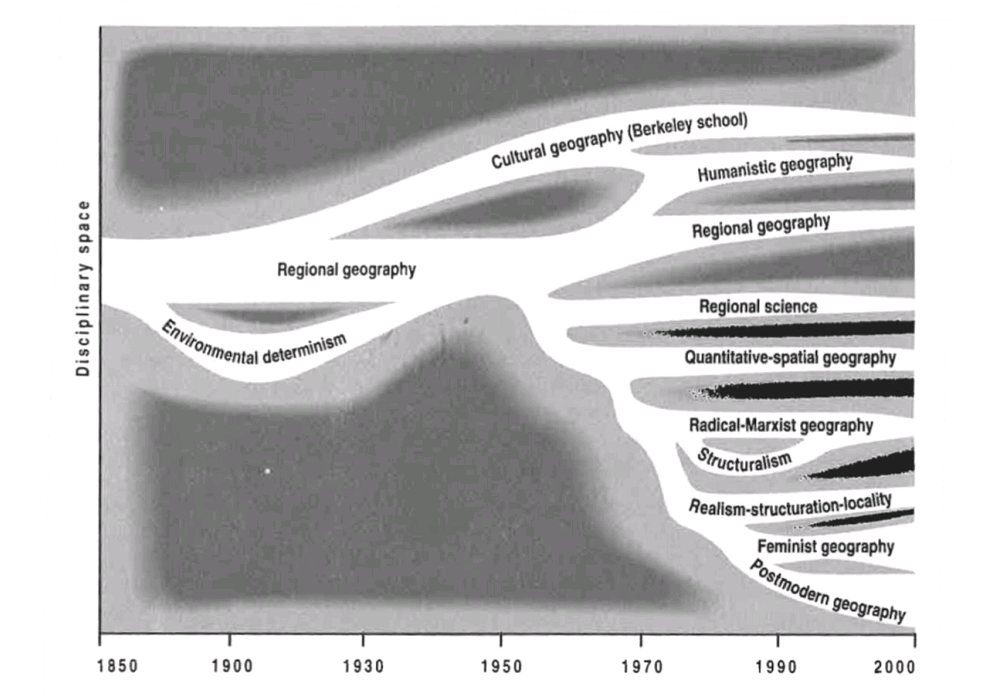
\includegraphics[width=30em]{geography_approaches.png}
\end{center}

%%%%%%%%%%%%%%%%%%%%%%%%%%%%%%%%%%%%%%%%%%%%%%%%%%%%
%											LECTURE 2
%%%%%%%%%%%%%%%%%%%%%%%%%%%%%%%%%%%%%%%%%%%%%%%%%%%%

\pagebreak\section{Theories of world-city formation}
\date{Octobre 4th, 2021}

The first session on world and global cities aims to:
\begin{itemize}
  \item Provide a framework to conceptualise and analyse cities under (economic) globalisation
  \item Give an overview of key theories of world-city formation dating back to the 1970s-1980s and onwards
  \item Introduce model-based approaches to the world-city network as a heuristic to map out how cities are positioned on global flows of capital, knowledge, and people
  \item Discuss a number of key critiques of the alleged ``world/global cities paradigm'', voiced from social constructivist and post-colonial positions
\end{itemize}

\subsection{Centrality of cities/city-regions in the global economy: Friedmann, Sassen, Scott}

How are cities central in the global economy? What does it mean to say that cities are powerful? 

\begin{outline}
	\1 Concentration of businesses, seats of corporate power, migration of elites to the city
	\1 Cities are administrative and political authorities
	\1 The city is a hub of ideas, culture, social influence, and knowledge transfer
	\1 Flows converge in cities, and flow between big cities: it's easier and faster to travel between cities than from a city to its periphery or towns. The substance of the flows can be knowledge, people, capital, commodities
\end{outline}

The five most powerful regions of Europe are Deltametropolis, Flemish Diamond, RheinRuhr Area, Ile-de-France, and Greater London.
There are multiple ways that we can measure the power, or influence, of such world-cities:

\begin{outline}
	\1 \textbf{Weight of area in national context}: the \textbf{GDP} is higher, and the density of population is higher\footnote{Higher than the European and national averages. This applies to the rest of the indicators.}
	\1 \textbf{Patents}: number of patents is higher. This indicates the level of social and technological innovations of a city
	\1 \textbf{Education}: the proportion of people educated at a high level is higher. This indicates a different labour market structure
	\1 \textbf{Employment by sector}: proportion of employment in services is higher, and proportion of employment in industry or agriculture is lower
\end{outline}

\subsubsection{John Friedmann, \textit{World City Hypothesis}}

\textit{tldr; world cities are basing points in a global (economic) urban system, organising and articulating production and markets}

\textbf{Why are cities economically central and powerful?}

There were predictions in the 1980s that ``the end of the city'' was coming, due to ICT and cheap mass transportation. Instead, these gave rise to new forms of uneven development related to \textbf{functional centrality} on a more global scale. People could travel from further distances and still work in the functional (city) centre, and have relationships with people from a longer distance.

World cities were inserted in a \textbf{global urban system}, in which urban processes that cross-cut national and regional borders are conceptualised: this insertion drives structural change in cities and renders some places powerful. We have to look beyond national urban systems, and start thinking about processes of \textbf{globalisation}, ie. on a global scale. A great part of economics became international, and only the global urban system can explain what is happening internationally. 

In this sense, world-cities are the base points to explain ``spatial organisation and articulation of production and markets'' (\textit{The World City Hypothesis}, Friedmann, 1986), ie. the geo-economic restructuring of the world.

There is a new \textbf{international division of labour} in the world. Companies offshore their production activities or relocate to (semi) peripheries to drive prices down because of cheaper labour markets, in order to stay competitive. There are new actors, TNCs and MNCs (trans- and multi- national corporations) that dominate and organise a global supply chain that is highly integrated\footnote{This complex, interconnected division of labour is illustrated by 1) the Evergreen container ship that blocked the Suez canal and blocked distribution of goods for a week, or 2) the lack of bicycles during the covid pandemic, when manufacturing plants had to close due to regional or national safety measures.} Given the importance of TNC/MNCs, mapping their headquarters can be used to locate world-cities. 

This illustrates that world-cities are sites for centralised \textbf{command and control} functions in a complex global economy. It implies a hierarchy connecting the core and the periphery, with core cities absorbing the surplus (and thus getting richer and growing in all dimensions)\footnote{This means that locations and cities will benefit unequally from this geography: the US (Global  North) producing in Argentina (Global South) will benefit the US, who extracts the profit, and disadvantage Argentina, who has a cheaper labour market}. But, (semi) peripheries can still hold local command and control functions.

\subsubsection{Sassen, \textit{The Global City}}

\textit{tldr; global cities are cities where APS (Advanced Producer Services) are produced for the international market; APS have control capabilities over global production, and they produce global financial markets}

Sassen writes at the same time as Friedmann, in a context of de-industrialisaiton (specially in NY, London, Tokyo) and fiscal crisis of the local state, and cities are trying to figure out what they might become.
Sassen focuses on the \textbf{shift to service economies}, especially finance services and auxiliary services in law, management consultancy, accounting, auditing, advertising, etc. These auxiliary services are called \textbf{advanced producer services (APS)}, they are not producing consumable goods, but rather goods that are consumed as they are produces (eg. legal advice).

Advanced producer services are embedded in global cities, and they have \textbf{control capabilities} to manage global production and produce global financial markets. There is a \textbf{labour market polarisation}, with high and low skilled labour forces surround APS, which results in the ``peripheralisation'' of the core (eg. sweatshops).

Sassen says that \textit{``global cities are sites for the production of specialised services needed by complex organisations for running a spatially dispersed network of factories, offices, and service outlets; and the production of financial innovations and the making of markets, both central to the internationalisation and expansion of the financial industry''}.

Global cities are connecting to the world of finance for investments, and growing the need for concentration and control. This geography is self reinforcing.

Why are APS concentrating in a limited number of cities? There are several interlocking \textbf{path dependencies}:
\begin{outline}
	\1 \textbf{Large services market}: there is access to firm/client relations, for out-sourced APS
	\1 \textbf{Labour market and associated culture}: a cosmopolitan elite and `yuppie' (young urban professional) culture is formed, since the 1980s
	\1 The most specialised and globalised APS firms need \textbf{synergies} with similar firms in the city, which creates an \textbf{APS complex}. For example, financial firms, ICT firms, advertising, management consultancy, accountancy, and legal services all need each other to some extent
	\1 The APS complex produces \textbf{cross-border connections} through a network of affiliates and other partnerships
\end{outline}

Even within the city, there are APS clusters. For example, the concentration of law firms in Avenue Louise and in the EU quarters of Brussels.

\subsection{Scott, \textit{Global City Regions}}

\textit{tldr; global city-regions are a complex assemble of cities/settlements/hinterlands that are interconnected via production networks, themselves oriented towards global economy}

Sassen's views of global cities as APS centres fits London, Hong Kong, Brussels, etc., but there are large-scale territorial entities like the Pearl River Delta\footnote{One of the most densely populated urban regions of the world, considered a megacity, and one of the wealthiest regions in China.} and the Bay Area, which have global power but are not cities. Many production processes don't need an `urban core'.

The need for centrality is applicable to \textbf{post-Fordist modes of production\footnote{Post-fordism is the idea that modern industrial production has moved away from mass production in huge factories, towards specialised markets based on small flexible manufacturing units}, where knowledge is central}. The concentration is a by-product of globalisation and technological innovations (cf. cognitive-cultural capitalism). 

So, not only APS need to be centralised. For knowledges that are not easy to de-centralise, proximity matters. For example 1) industries in which it is important to communicate with clients face-to-face, or 2) tailored, just-in-time delivery. Concentrating an activity in one area also makes it easier to receive federal/public investments (ie. investments drive centralisation).

\textbf{Global city-regions} are a complex ensemble of cities/settlements/hinterlands, that are interconnected via multiple production networks, which in themselves are oriented towards the global economy. APS firms can still be used as a general indicator of the globalisation of Global City-Regions, as they produce the tools to enable proper functioning in a global economy.

\subsection{Mapping world city networks}

Comparing the importance of urban connections (eg. London/Hong Kong vs Paris/Tokyo) is difficult when using available data sources, and without using a secondary data source or creating new data.
This is because there is a research gap regarding world-city networks.
Secondary data could be information on inter-city transportation or information flows (eg. flows of airline passengers). New data collections could be developing a methodology to use specific attribute data to assess inter-city relations (eg, the GaWC-heuristic).

Are airline flows a good way to measure global economic influence, and thus helpful to map the world-city network?
\begin{outline}
	\1 Some cities which are not global-cities have airports, and maybe vice versa
	\1 People travel for leisure, which may tell us something about the local economy but not about the influence of the city's economy on a global scale
	\1 A lot of goods are moved by other means than air, eg. water or land
\end{outline}

Therefore, we need a \textbf{new metageography} of spaces of flows. This would be a new socio-spatial structure.

The GaWC (Globalisation and World Cities) heuristic is an example of a new way to gather data\footnote{See \url{https://www.lboro.ac.uk/gawc}}. The starting point is the presence of international APS firms, that is used as a general indicator for command and control functions of cities. Since APS firms have office networks that comprise of the most important cities in the global economy, we make the core assumption that inter-city relations can be assessed based on the APS firms being present in multiple cities. $\rightarrow$ we measure the connectivity of cities.

APS don't represent all of the global economics, but they represent strategies of the command-and-control of APS firms. 

\subsection{Critiques and complementary views}

The GaWC heuristic is a powerful tool to map and spatially analyse the global connections of world/global cities, but has been criticised from various angles: post-colonial, social-constructivist, political-economy, and financialisation perspectives.


\begin{outline}
	\1 \textbf{Post-colonial critique}: there is a western bias in the knowledge production of urbanisation, people are dropped off the map of urban studies research. 
		\2 Off the geographical map refers to (world) cities in the Global South
		\2 Off the conceptual map refers to the focus on a limited number of economic processes, and ignoring equally important inter-urban connections
		\2 World cities research ignored the role and position of `ordinary' cities in the global economy,  or reads them in light of Eurocentric global city theories 
		\2 Tendency in urban studies to reject world/global city theory as only befitting the Global North, but not on the basis of a sound argumentation: non-representation as a `result', not a `neglect'
	\1 \textbf{Social-constructivist critique}: stresses the political natural of world-city formation and its often un-debated consequences
		\2 Post-modern knowledge theory: world cities are not a `given' but a product of global and local forces, and crucially mediated by acts of representation
		\2 For example, London is a globalised financial service centre, but the way we perceive it is the result of how financial elites and politicians have been projecting London the world stage as a `hegemonic' neoliberal growth strategy (Thatcher), which hides other realities like the low-skilled migrant labour
		\2 There are also pro-City policies like subsidising infrastructure, higher interest rates...
	\1 \textbf{Political economy critique}
		\2 State rescaling: a spatial restructuring of the nation-state due to globalisation, which changes the scale to supranational and subnational levels
			\3 There are new governance structures and a new spatial articulation of the state, but also a shift from managerialism to entrepreneurialism (Harvey, 1989). This is particularly evident with urban policy makers prone to the discourse of inter-urban competition
			\3 The emergence of global cities is a corollary of the city-centredness of global accumulation regimes, mediated by global-city building agendas
	\1 \textbf{Financialisation}: GaWC heuristic is a powerful shorthand for the geographies of world/global cities, but world-city functions are often assumed instead of researched
		\2 The leading assumption from Friedmann and Sassen is that APS provide a ``seamless service under conditions of globalisation'' (Taylor, 2004), ie. allow the combination of capital and labour on a global scale
		\2 However, since the 1970s there has been an intense deregulation of financial markets and growth of private capital flows (eg. `Big Bang' in London, 1987). These are processes of financialisation, ie. finance capital logics become dominant
		\2 As a consequence firms have not only globalised, but also financialised (listed and traded on the stock market). APS complexes are obligatory passage points, holding a monopoly position in the context of over-accumulation, legitimising risk-taking that led to the Global Financial crisis (Bassens, van Meeteren, 2016)
		\2 Eurobonds
		\2 Tax evasion
\end{outline}

\subsection{Key words}

World cities
World city-regions
Global urban system, global economic system
GaWC
Command-and-control function of cities

%%%%%%%%%%%%%%%%%%%%%%%%%%%%%%%%%%%%%%%%%%%%%%%%%%%%
%											LECTURE 3
%%%%%%%%%%%%%%%%%%%%%%%%%%%%%%%%%%%%%%%%%%%%%%%%%%%%

\pagebreak\section{Polarisation in World/Global Cities}

This second session on world and global cities discussions the connections between the positionality of cities on global circuits of value and their internal social and economic structure:
\begin{itemize}
  \item Applies Harvey's framework to analyse urban  entrepreneurial export-base enhancing strategies
  \item Focuses on the polarisation debate, which has centred on the mechanisms that produce income \& professional divides, the contextual factors that mediate such polarisation processes, the role of high/low-skilled migration, gentrification, etc.
\end{itemize}

\url{https://www.youtube.com/watch?v=qOP2V_np2c0&ab_channel=RSA}

\subsection{Polarisation}

\textit{tldr; polarisation is a class division that is reproduced through space, and is stronger in global cities}

Income disparity looks different in different cities. Chicago, Detroit, LA, Miami, New Orleans, SF, NYC, all have different, contextual landscapes of polarisation.

Polarisation is the reality of \textbf{class division}. \url{https://www.opportunityatlas.org} is an income map that traces neighbourhood effects, based on census data. The \textbf{neighbourhood effect} is the idea that where you are born, predetermines your life. This is due to the amenities, infrastructure, opportunities associated to the geographical location.

Polarisation is one of the starting point of debates in global cities: it raises the questions about \textbf{how class divisions in cities are reproduced in/through space, but also why there is a deep polarisation in key nodes in the global economy}, ie. in world/global cities.

Picture LA, a `citadel' city where polarisation/segregation are both horizontal and vertical (there are no wealthy people residing on the ground floor). Wall Street in LA is a poor neighbourhood in decline, or a `zone in transition', yet it is contrasted with nice hotels. This says to people that `those who have nothing to do here, should not be here'.

\subsubsection{New York City}

We can see how NYC's polarisation patterns have evolved in the last decade, since the 2008 recession: \textbf{polarisation and income distribution gaps have increased}. 

The median family income has fallen\footnote{Income can be equated to labour}, and the decline in income is steeper in NYC than in the state of NY. The share of total income going to the top 1\% continues to increase (it only declines during a financial crisis but quickly rebounds), such that the top 1\% own over 40\% of the total income and the income of the lowest household is \texttildelow17.5\% of the top earners' income. And the gap in increasing.

\textbf{Productivity has increased but wages have not}: for 1 hour of work, an extra 14\% is produced, but the wages have not proportionally increased. The profit is not going to the workers, and a full-time worker at a minimum wage now lives under the \textbf{poverty line}.

\begin{center}
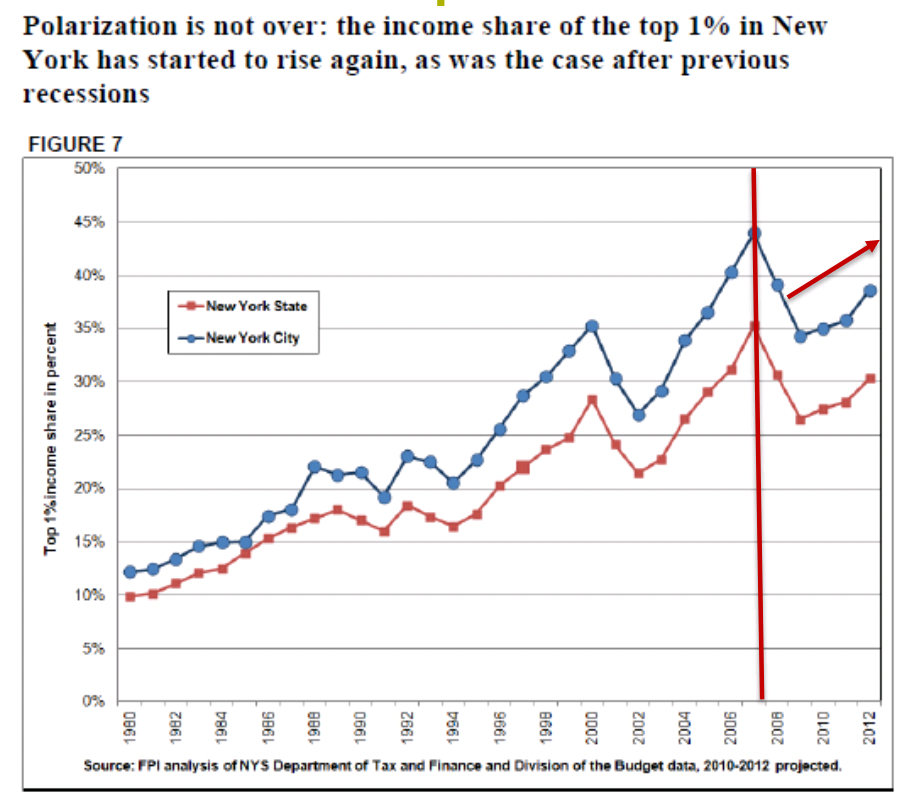
\includegraphics[width=23em]{nyc_income_gap}
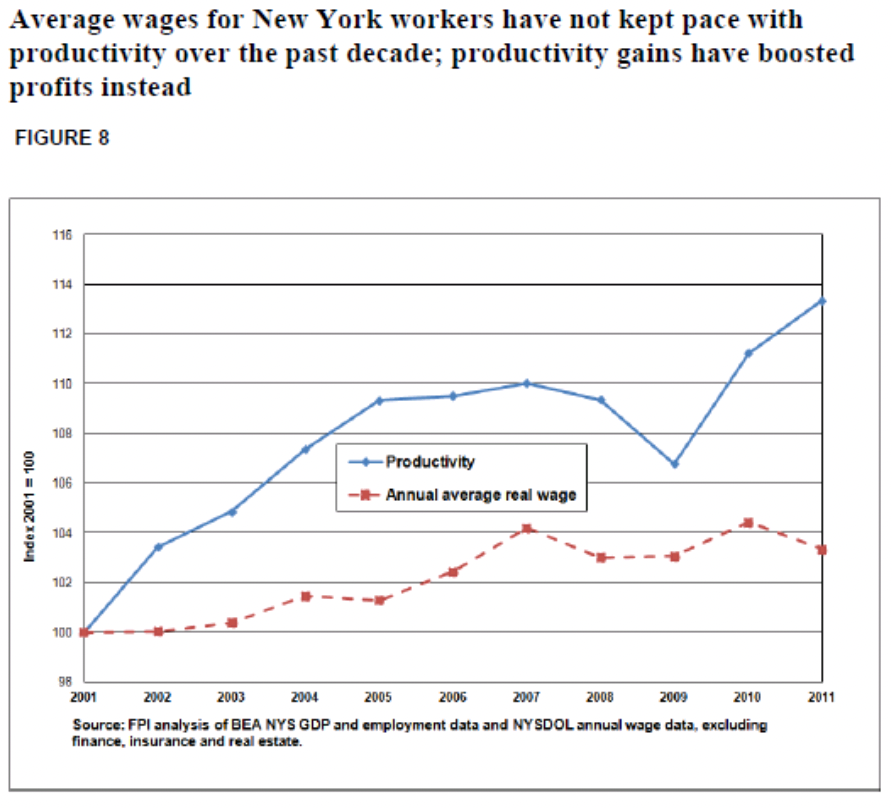
\includegraphics[width=23em]{nyc_productivity_gap}\footnote{Fiscal Policy Institute report, \textit{Pulling Apart: The Continuing Impact of Income Polarisation in New York State}}
\end{center}

\subsubsection{Why is it that world/global cities have become so polarised?}

\begin{outline}
	\1 Large companies with a lot of capital are subsidised
	\1 Unequal income distributions, where rich companies are getting richer
	\1 Companies are looking for the fastest way to make money, ie. they employ at the lowest wage possible. It's a corporate strategy to not care about the general welfare of the workforce
	\1 The state is not taking the role of creating regulation and (welfare) policies
	\1 Extra money ``floating around'' goes into financialisation, as can be seen with the gap in productivity (profit) and wages 
	\1 Companies can remove workers who want higher wages, because there is enough demand for such low-wage jobs
	\1 A worker needs to be produced in a ``social way'', including education, health,... (social reproduction) which happens in cities
	\1 Poverty blaming does not help with polarisation, eg. Benefit Street
\end{outline}

\subsection{Conceptualisation}

The main explanation for why polarisation exists, is because of economic restructuring (this is mostly about North-Atlantic cities).

Some conceptualisations:
\begin{outline}
	\1 ``Dual cities'', Mollenkopf and Castells, 1991
	\1 ``Divided cities'', Fainstein et al., 1992
	\1 ``Quartered cities'', Burgers, 2002
	\1 ``Polarized cities'', Sassen, 1991; Friedmann 1986
\end{outline}

\subsubsection{Economic restructuring}

The crisis of North-Atlantic Fordism in the 1970s led to an economic restructuring. With Fordism, there was a deal between the companies and workers, that they would get a wage allowing them to purchase the items they were manufacturing. However, productivity couldn't keep up with wages. This entailed:

\begin{outline}
	\1 \textbf{A relocation of production}, ie. offshoring and decentralisation made possible by \textbf{globalisation and the new international division of labour} (NIDL)
	\1 \textbf{The deindustrialisation of the core}: production activities in cities declined
	\1 \textbf{Structural unemployment}: as cities lost their functions, poverty rose and became characteristic of cities
	\1 \textbf{Shift towards fiscal austerity}: the tax base declined
	\1 \textbf{Market rationality and privatisation}: the state interfered less and encouraged privatisation (market deregulation which enriched companies), and shifted towards neoliberalism (Thatcher, Reagan)
	\1 \textbf{Declining power of the state to control multinational capital}: this power shifts to multinational companies
	\1 \textbf{Self fulfilling prophecy of interurban competition}: policy makers are trying to become entrepreneurial, and instead of being fair, start to be competitive
\end{outline}

Harvey (1989) proposes four ``entrepreneurial'' strategies to navigate this crisis: production, consumption, redistribution, command and control

\subsubsection{Production}

Policy makers create or exploit particular advantages for the production of goods and services:

\begin{outline}
	\1 Attracting public and private investments into physical and social infrastructure, to strengthen the economic base 
	\1 Stimulating new technologies, venture capital...
	\1 Reducing local costs with tax breaks, cheap credit...
	\1 Reducing ``excessive'' labour costs or investing in highly educated labour force
	\1 Stimulating a mix of related activities and creating agglomeration economies, eg. Silicon Valley
	\1 \textbf{Form}: clusters and edge cities
\end{outline}

\subsubsection{Consumption}

The city's position in the spatial division of consumption should be improved:

\begin{outline}
	\1 Make people want to spend money in your city: through tourism, retirees, local consumers
	\1 Residents rarely see an increase in their wages, despite the attraction of money in their city
	\1 There's an increased credit, and a dependence on banks to finance consumption
	\1 Attract high income jobs (managerial, CEO...) and their conspicuous consumptions
	\1 \textbf{Form}: the socio-spatial structure is affected by consumerism, visible by gentrification, cultural innovation, upgrading of urban environment (starchitecture), consumer attractions, spectacle, heritage, city branding/marketing
\end{outline}

\subsubsection{Redistribution}

There is a competition for the (supra)nationally distributed surplus. Cities and regions compete with each other to attract investments. The surplus comes from the economy, and not the government budget. Especially under austerity, which cuts government budget and makes the surplus allocation problem greater.

Who competes for surplus?

\begin{outline}
	\1 Military/defense investments in the US
	\1 EU countries for EU money
	\1 Urban renewal projects in Flanders
\end{outline}

\subsubsection{Command and Control}

A specific kind of investment in connectivity, to assume control in high finance, government, and information gathering/processing:

\begin{outline}
	\1 Investment in connectivity infrastructure, both physical and digital
	\1 CBD-development and office space strategies
	\1 Investment in high-skilled labour markets and education (universities, business schools,...); companies sponsor finance programs for employees
	\1 \textbf{Form}: a dynamic in world/global cities and their monopoly spaces (eg. Wall Street, the City of London)
\end{outline}

\subsection{Polarisation thesis}

Main authors are Friedmann \& Wolff (1982), Friedmann (1986), Sassen (1991)

The key trend is the change in economic base, leading to a decline in well-paid manufacturing jobs (exodus) and a growth in service jobs (formal/informal).

This entails an influx of high salaried people, with high spending power (the highly-skilled, highly-paid, upper circuit, upper social strata). This in turn generates a demand of low paid jobs to cater to them  and their conspicuous consumerism (low skilled, low paid, underclass, the remaining social stratum).
This transforms the labour market, such that there is a growth of \textbf{jobs at the top and bottom} of the job ladder, but a decrease in demand for jobs in the middle. The informal economy and informal workers also grow.

\begin{center}
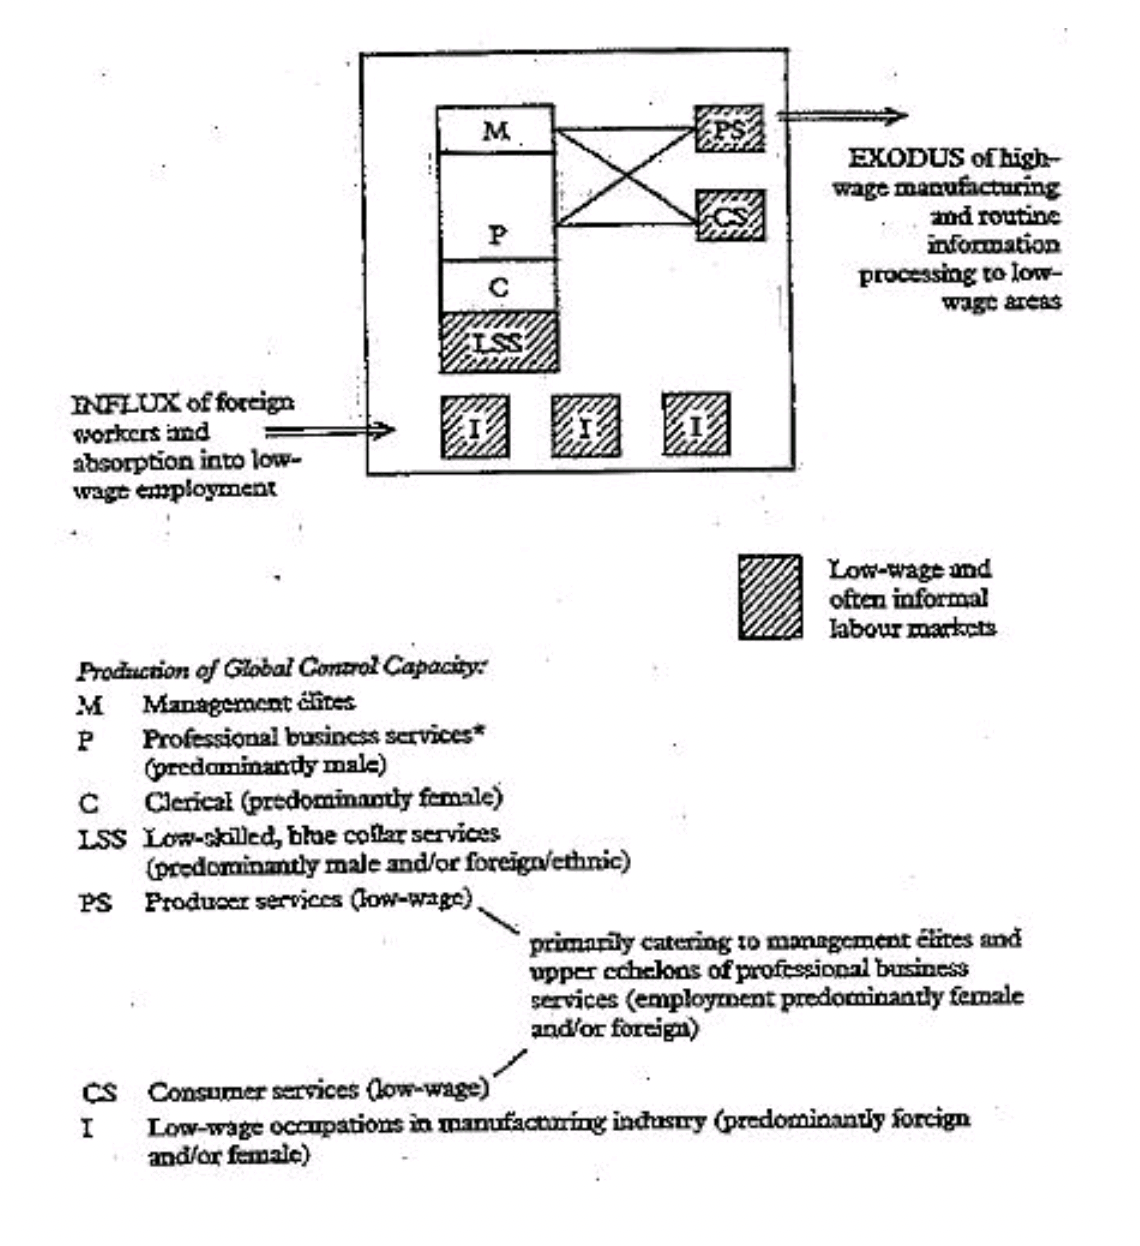
\includegraphics[width=40em]{polarisation_thesis}
\end{center}

\subsection{Labour Market Globalisation}

What sets global cities apart is their \textbf{globalised labour market}. There is a growing role of high-paid and low-paid migrants in the urban economy, this divide is often articulated along ethnic lines (``expats''\footnote{Debate in Belgium about how to tax expats, who currently enjoy a low tax rate} vs. ``immigrants'').

The growth of the supply of low-skilled/deskilled workers causes a downward pressure on wages. These are people who did not have, or no longer have (ie. having lost, or not recognised) qualification from their country of origin.

This creates a large pool of people who do not have power to make demands on their wages, and the pool is large enough that workers can be replaced by others who are willing to work for these low wages.

An example of low-skilled jobs are \textbf{3D jobs} (dirty, demanding, dangerous/difficult) originally were paid higher wages in order to attract workers. Now, low-wage jobs are for those otherwise excluded from the labour market.

There is growing \textbf{informality and ``peripheralisation at the core''} (Sassen-Koob, 1982). Exploitation does not only take place in the Global South: it also takes place in the Global North (ie. the global cities, the core) where people from the Global South (the peripheralised) live.

Immigration lead to the expansion of `informal', `floating', or `street' economic activities, such as sweatshop manufacturing, off-the-book childcare, and other unregistered, non-taxpaying activities. You need some knowledge to be able to access the market place, or you are excluded and must find informal work.

\subsubsection{Urban Elite Networks}

A way of measuring the connection between cities, by looking at the membership overlaps across the board of directors (one member sitting in multiple boards).
 
 \subsubsection{New forms of industrial exploitation}
 
Sweatshops are reminiscent of old-forms exploitation. They are small units in secluded spaces, they function with subcontracted deals which makes it hard to know who is actually contracting, and workers are paid by the pieces or by weekly contracts. This is highly precarious work and hard to regulate.

Sweatshops have re-emerged in the new industrialisation age (20-21st century), which is made possible by the absence of labour rights protection. They are always located in the global peripheries.
 
\textbf{Thus, global city formation is made possible by the absence of regulation in the periphery.}
 
\subsection{Criticism}

The two main criticisms are:

\begin{outline}
	\1 \textbf{Universalising and generalising tendencies}: started in London, NY, Tokyo, and is considered universal, but is it the case? 
		\2 The thesis projects this logic: economic restructuring + globalisation $\rightarrow$ HQ + APS functions $\rightarrow$ income + professional polarisation $\rightarrow$ socio-spatial polarisation
	\1 \textbf{Simplistic theory}: polarisation theory is elegant but reduces the complexity of what is going on. Occupational and spatial structures need to be studied in detail. Professionalisation and mobility could also help explain socio-spatial inequalities
\end{outline}

\subsection{Occupational Structure}

\textbf{Polarisation vs. professionalisation}: London's high-income jobs are growing, but this is not necessarily combined with a growth of low-paid jobs. The reason is that the labour market is ``upgrading'', such that people with the required qualifications for highly skilled jobs are moving up the social ladder, which expands, not declines, the middle class.

Plus, a more generous welfare state curbs extreme polarisation (eg. no sweatshops, presence of minimum wage).

The main source of inequality emerges from labour market \textbf{exclusion} and how labour markets intersect with \textbf{gender and ethnicity}. For example (in NY and London), the upper stratum of the executive and professional is dominated by white males; racial and gender discrimination is restricting access of certain groups to highly paid jobs even if they possess required skills; ethnic groups are concentrated in specific parts of the economy, third of London's Filipino population is in health/social care, and Brazilians in cleaning services.

\subsection{Spatial Structure}

\begin{outline}
	\1 To what extent is polarisation a statistical artefact?
The middle class is \textbf{suburbanising}, so maybe the middle income job disappearance is an of artefact as suburbanisation, and thus the entire metropolitan area needs to be taken into the analytical scale, not just the city centre $\rightarrow$ scale matters
	\1 Higher incomes drive demand for high-end housing. This ignites a process of a return to the city and ultimately, (super) gentrification pushing out middle classes
		\2 Brooklyn
		\2 Brussels' evolution of migrant populations: the Moroccan population has grown in the north-west ``poor crescent'', but Europeans and expat populations have grown in the south-east part of city. This is caused by Belgian policies, which promoted Brussels to North Africans as a prosperous city; when industry declined in Brussels, the immigrant families concentrated in the north-east.
	\1 Occupational and income restructuring can take many spatial forms. Need to look at pre-existing structures of the city and its path-dependencies
\end{outline}

\subsection{Three-layer model}

A three-layer explanatory model is required for analysing inequality in cities (Burgers and Musterd, 2000)

\begin{outline}
	\1 Macro-level: a level of global change, referring to economic restructuring, and the increasing mobility of capital, people, commodities and information
	\1 Micro-level: an individual level, referring to the change in labour market opportunities of individuals in a specific local context
	\1 Medium-level connecting the macro and micro-levels, the global and the local
		\2 Subcultural differences among ethnic groups in labour market access
		\2 National institution differences, eg. corporatist social democratic welfare states in Europe provided strong employment protection and benefit systems, which had a moderating impact on the outcomes of economic structuring in the 1980-90s; vs. the liberal welfare state of the USA showed more pronounced levels of inequality due to the loss of jobs and income
		\2 Different urban trajectories, related to urban functions and positionality; industrial towns (eg. Charleroi, Detroit) vs. administrative centres or command-and-control centres
\end{outline}

\subsection{Conclusion}

The gap between the rich and poor is expected to expand. 

\begin{outline}
	\1 \textbf{Austerity}: the permanent state of austerity means stagnating income and declining subsidies, which generates very unstable conditions for lower incomes
	\1 \textbf{Flexibilisation of the labour market}: increased levels of long-term unemployment, and flexible low-wage jobs put a large portion of the population close to the edge of financial insolvency
	\1 \textbf{Migration}: renewal of reserve army of labour through migration, if social policies are not put in place the environment for exploitation will not disappear
	\1 \textbf{Political wealth}: return of patrimonial capitalism, a rentier class banking on wealth and not labour. It matters more who your parents are, your return on investments, than the choice of your profession and your amount of labour
\end{outline}

The function of cities is transforming, and they are becoming `safety deposit boxes' for the people who rely on wealth. For example, in London entire neighbourhoods like Knightsbridge and Chelsea are owned by people who live in the Middle East; Shell companies owning 30 million \$ apartments in Manhattan, to maintain their wealth in a given place, but these buildings are empty.

Thus, de-urbanisation is taking place in global cities, where there are growing numbers of empty shells, and neighbourhoods

%%%%%%%%%%%%%%%%%%%%%%%%%%%%%%%%%%%%%%%%%%%%%%%%%%%%
%											LECTURE 4
%%%%%%%%%%%%%%%%%%%%%%%%%%%%%%%%%%%%%%%%%%%%%%%%%%%%

\section{Urban segregation: patterns and causes}

\textit{October 25th, 2021 - Nick Schuermans}

\subsection{Classical land-use models}

Land use models, or models of urban form. Elements of all these classic models can be identified in many large Western cities.

\subsubsection{Burgess' land use model, 1925}

Burgess was trying to understand what cities looked like, and what kind of groups can be found where.
He found 5 concentric rings: the loop (CBD), zone of transition, zone of working class, suburban zone, commuter zone.

\begin{outline}
	\1 \textbf{Loop, or CBD}: Chicago had an elevated metro track that ran in a loop; place with shopping, offices, HQs, theatres... ie. the functions that are able to pay the highest price for this central location. They need to draw workers/consumers from all corners of the city, thus need to be in the loop
	\1 \textbf{Zone in transition}: factories that rely on labour coming from different parts of city, but who are not able to pay as much rent as the businesses in the loop; also residential, for first generation immigrants who cannot yet afford to live further out (eg. Little Sicily)
	\1 \textbf{Working class zone}: `respectable' working class neighbourhoods (eg. Belgians, Russians, who had been able to climb social ladder and move away from factories)
	\1 \textbf{Suburban zone and Commuter zone}: better, middle-class residences and commuter belt
\end{outline}

The reason there are five rings, is because of the \textbf{bid rent theory}. It explains that different groups of people are able to pay (afford) different amounts of rents. The centre, being the most attractive, has the highest rents and only firms are able to afford them. The further away from the centre one goes, towards the suburbs, the less dense the areas are and thus the lower the rents (to a certain extent, and with exceptions).

The concentric model was created in 1925, which is around the time that Chicago was going through an exponential growth. Thus, Burgess' model is that of \textbf{a growing city}. It tries to understand how the growth works in terms of population and the built environment.

Assumptions and principles of the model:

\begin{outline}
	\1 Cultural and social heterogeneity of the population
	\1 Commercial and industrial base to the economy of the city
		\2 But, other industries can dominate the city, eg. tourism, heritage, religious/pilgrimage
	\1 Private ownership of property and economic competition for space
		\2 But, there exists(/existed) planned economies under communism
	\1 Expanding area and population of the city
		\2 But, some cities are marked by shrinkage, eg. Detroit
	\1 Transport is equally easy, rapid, and cheap in every direction within the city
		\2 But, this is almost never true
	\1 The city centre is the main centre for employment, thus most valuable
		\2 But, eg. airports are also hubs of employment and consumption
	\1 No districts are more attractive than others because of differences in terrain
		\2 But, coasts, mountains, and other terrains influences attractiveness 
	\1 No concentration of heavy industry
	\1 No historic survival of an earlier land-use pattern in any district
\end{outline}

Thus, it's obvious that these assumptions do not apply to any real city, and Burgess acknowledged it. The model is an ideal type, a simplification.

\begin{center}
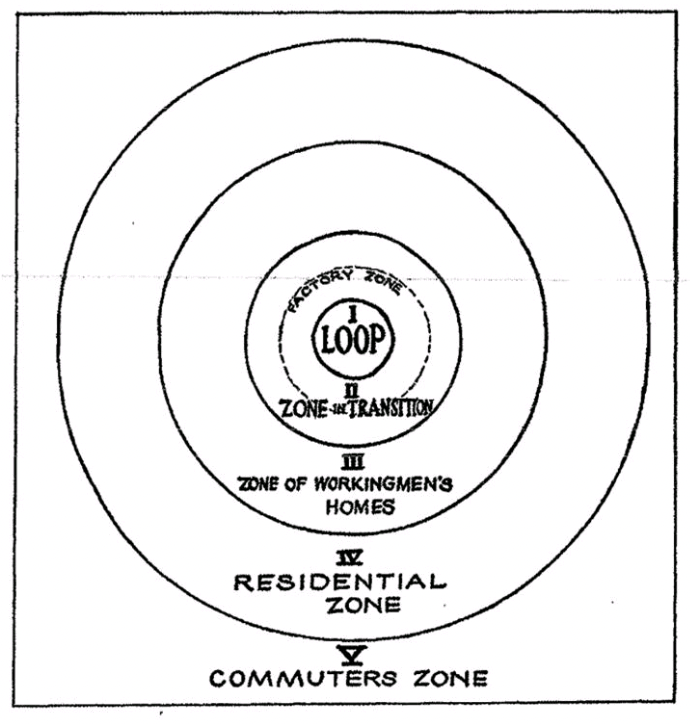
\includegraphics[width=30em]{burgess_model}
\end{center}

\subsubsection{Hoyt's sector model}

Between 1925-1939, the depression and economic crisis affected the US and less people were willing to move there. Thus, Hoyt was theoritising of a model where cities grow slowly, and the car plays an increasingly important role.

The sector model reflected the strong core (CBD) around which sectors are organised. When the city grows, or a certain group of people grows, these sectors grow outwards. There is a focus on class, rather than group of migrants.

\begin{center}
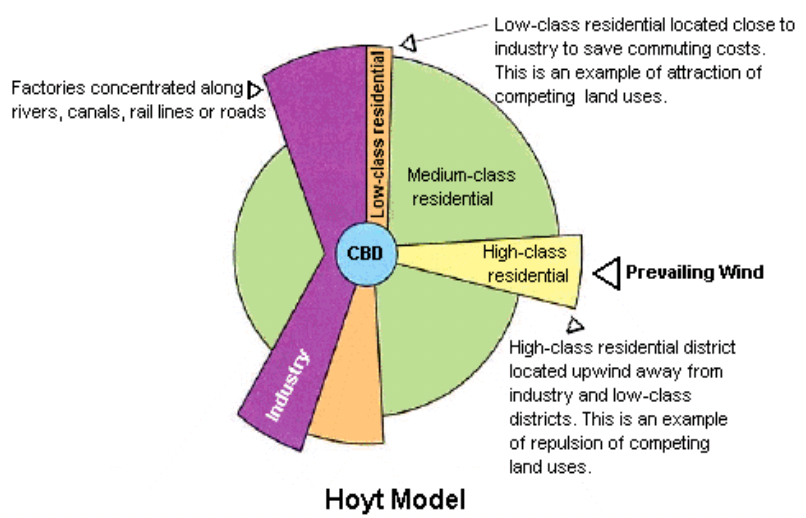
\includegraphics[width=30em]{hoyt_model}
\end{center}

\subsubsection{Harris and Ullman's multi-nuclei model}

A multi-nuclei model, where cities have a CBD but also other strong areas, with business (eg. river side industries) and other institutions (eg. universities).

\begin{center}
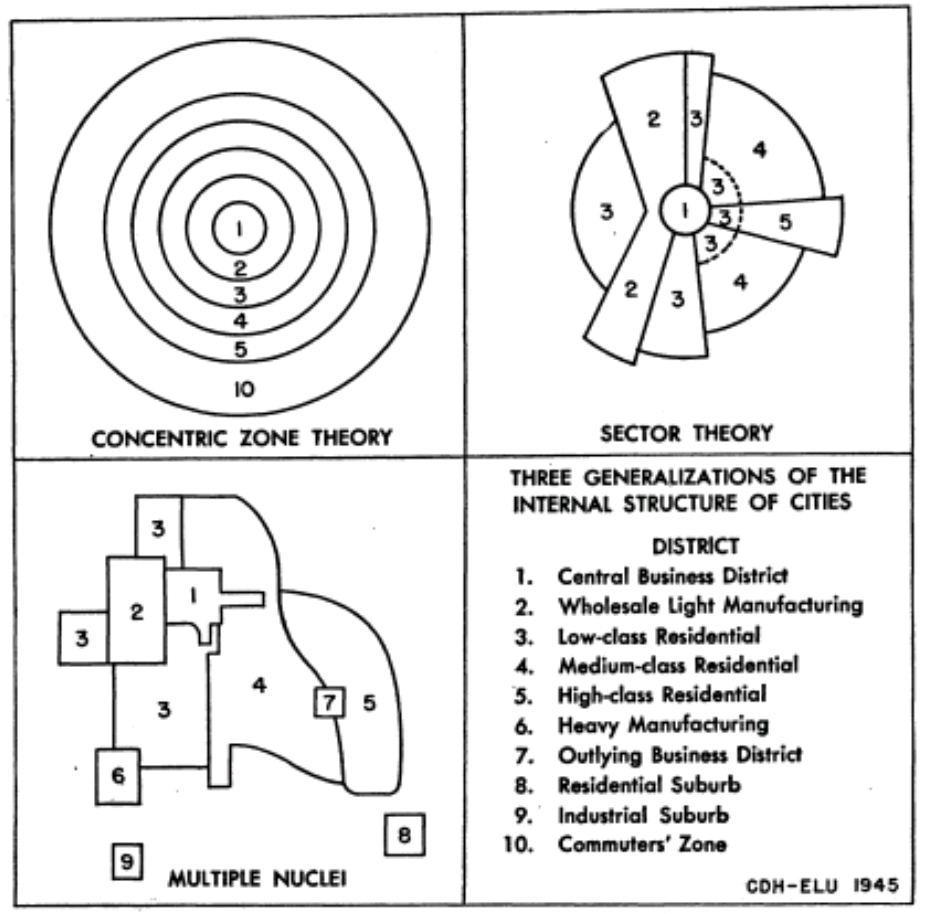
\includegraphics[width=30em]{harris_ullman_model}
\end{center}

\subsubsection{Alternative models}

The British city (Kearsley), the Chinese city (Burns), the African city, (De Blij), LA in 1990s (skid row, gated suburbs, Davis), the post-socialist city (Tallinn).

\subsubsection{Conclusion of classic land use models}

\textbf{Local features impact urban form} (topography, water bodies, prevailing wind direction, economic base of the city, migration patterns...) and \textbf{local policies impact urban form} (transport system, state interventions in housing, restrictions on mobility, strategies to counter inequalities...)

Thus, every model of urban form has its birthmarks, and is from a specific place and time. They need to be situated as such. We also need to \textbf{provincialise} theories about urban form and growth.

\subsubsection{Exam question - classic land use models and alternatives}

Exam question 2016: The figure below describes the model of the South African post- apartheid city by Christopher (2001). You can assume that the rich live in low density suburbs; the poor in high density suburbs and flats and hostels for male workers. +++ is a rail line; ---- represents a main road. Which elements of Burgess’, Hoyt’s and Harris and Ulman’s models of urban land use do you recognize in this model? (/5)

\[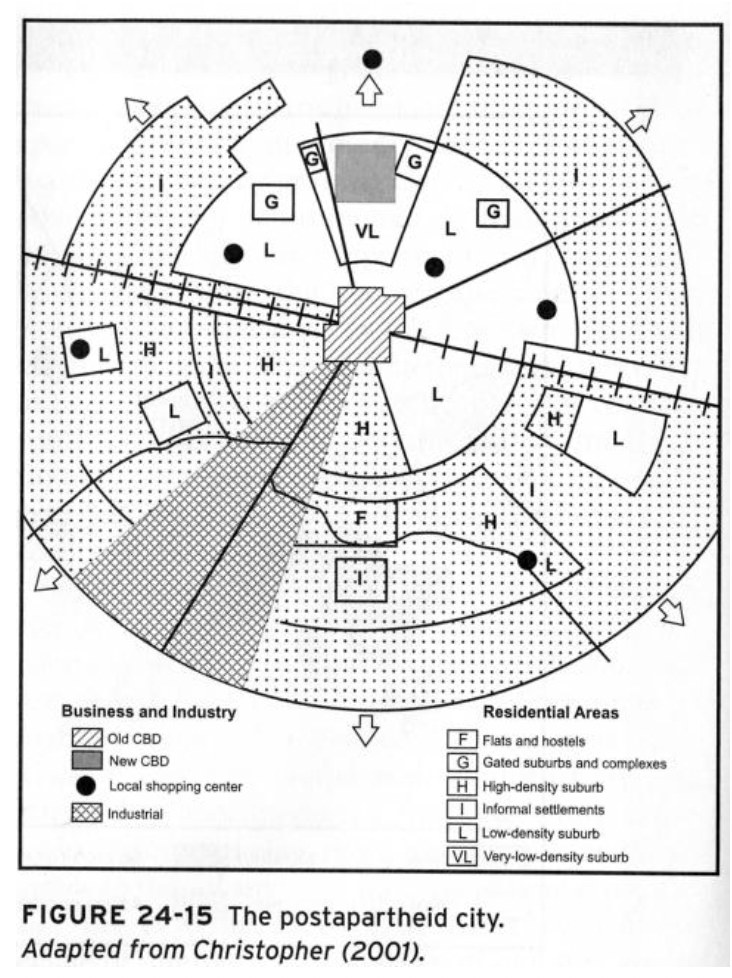
\includegraphics[width=15em]{examq_apartheid_model}\]

\subsection{Patterns of segregation}

\subsubsection{Massey and Denton’s five dimensions of segregation}

Segregation here is focused on \textbf{residential segregation}. It is the degree to which two or more groups live separately from each other, in different parts of the urban environment. Massey and Denton’s (1988) describe five dimensions of segregation: evenness, exposure, concentration, centralisation, and clustering.

\begin{outline}
	\1 \textbf{Evenness} is the differential distribution of two social groups, among areal units in a city; a minority group is said to be segregated, if it is unevenly distributed over a given area.
	The \textbf{index of dissimilarity} measures the unevenness in population across space. If an index is low, it means that the population is evenly distributed (ie. less segregation), whereas if an index is 100, the population is unevenly distributed (ie. high segregation). 
	\1 \textbf{Residential exposure} is the degree of possibility of interactions or contact, between minority and majority groups within geographic areas of the city; the degree of which these groups confront each other by virtue of sharing a common residential area
	\1 \textbf{Concentration} is the amount of physical space occupied by a minority group in the urban environment; groups that occupy a small share of the total area within a city are said to be residentially concentrated
	\1 \textbf{Centralisation} is the degree to which a group is spatially located near the centre of an urban area
	\1 \textbf{Clustering} is the degree of spatial clustering exhibited by a minority group, ie. the extent to which areal units inhabited by minority members adjoin one another, or cluster, in space
\end{outline}

\subsubsection{Scale matters}

Looking at segregation at different scales, give you very different results as to how segregated a city is. 

\begin{center}
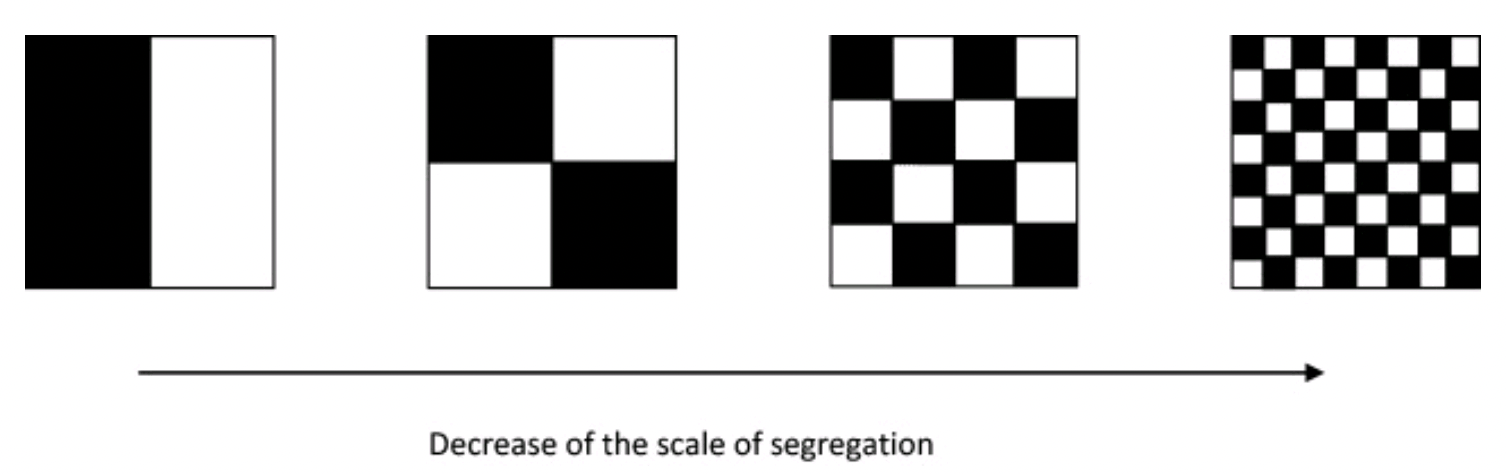
\includegraphics[width=30em]{segregation_scale}
\end{center}

\subsubsection{Exam question}

Exam question 2017: Use the three most relevant dimensions of Massey and Denton’s (1988) five dimensions of segregation to discuss socio-economic segregation in Brussels. Define each dimension of segregation you are using.

\[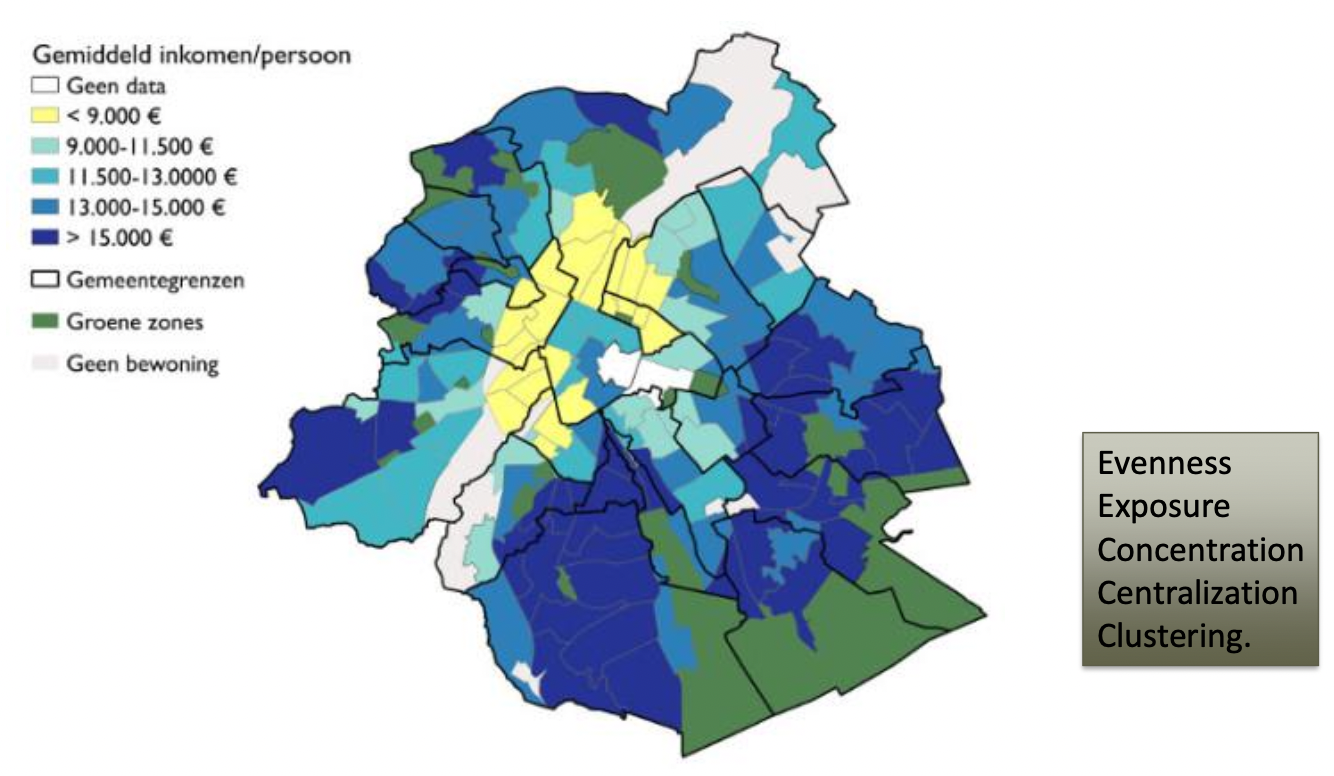
\includegraphics[width=30em]{examq_segregation_dimensions}\]

\subsection{Causes of segregation}

Why do different population groups occupy different parts of the city? There are many threads of geographers, with different opinions.

\begin{outline}
	\1 \textbf{Quantitative spatial geography}
		\2 \textbf{Ecological models} of the city
		\2 eg. ``urban metabolism'', ``natural forces''. It views the urban environment as a natural area, with a homogeneous character, characterised by a pattern of expansion (physical growth of the city) $\rightarrow$ competition (among land uses) $\rightarrow$ invasion (of the most desired parts of the city) $\rightarrow$ succession (of existing land uses)
	\1 \textbf{Radical-Marxist geography} 
		\2 Aims to understand the flow of capital, and the accumulation regime; how segregation fits within the accumulation of capital (Harvey)
		\2 The ecological models are considered to be mechanistic, ideological and devoid of ethical content
	\1 \textbf{Neo-Weberian} approach
		\2 Constraints due to financial resources, cognitive resources, political resources, social resources, and present housing condition
	\1 \textbf{Behavioural geography}
		\2 Based on people's reasoning and preferences around living in a certain environment over another; there is a focus on the demand side of the housing market, which is closely tied to the family life-cycle
		\2 It can be done with an ethnic lens
	\1 \textbf{Post-modern geography}
		\2 The meaning of housing, and how this affects one personally, because housing is not just structural, but also about feeling at home
		\2 Raises questions like, what does moving to the suburbs do to a middle-class family? how does social mobility impact people? why do gentrifiers move back to the city centre?
		\2 It's all about having an identity, and how people understand and distinguish themselves from one another; gentrification is something that's promoted by the cities
\end{outline}

\[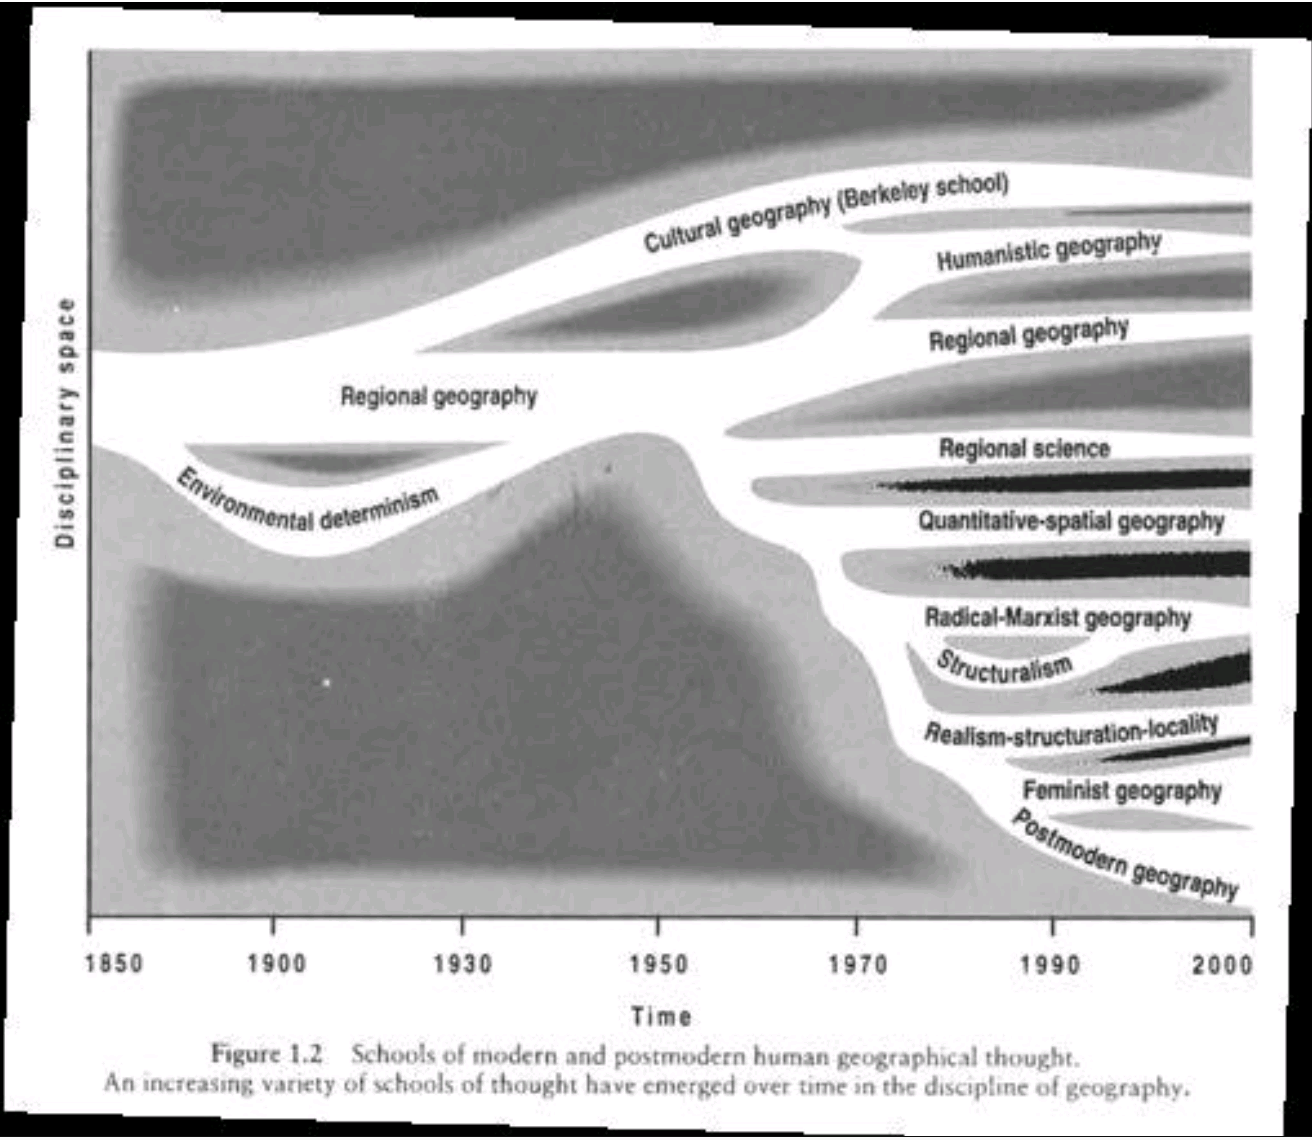
\includegraphics[width=30em]{geographer_types}\]

\subsubsection{Exam question}

Exam question 2017: Below, you can find a map with the distribution of people of Turkish and Moroccan origin in the city of Antwerp. How would urban geographers from different schools of thought explain the patterns on the map? Refer to at least three traditions.

\[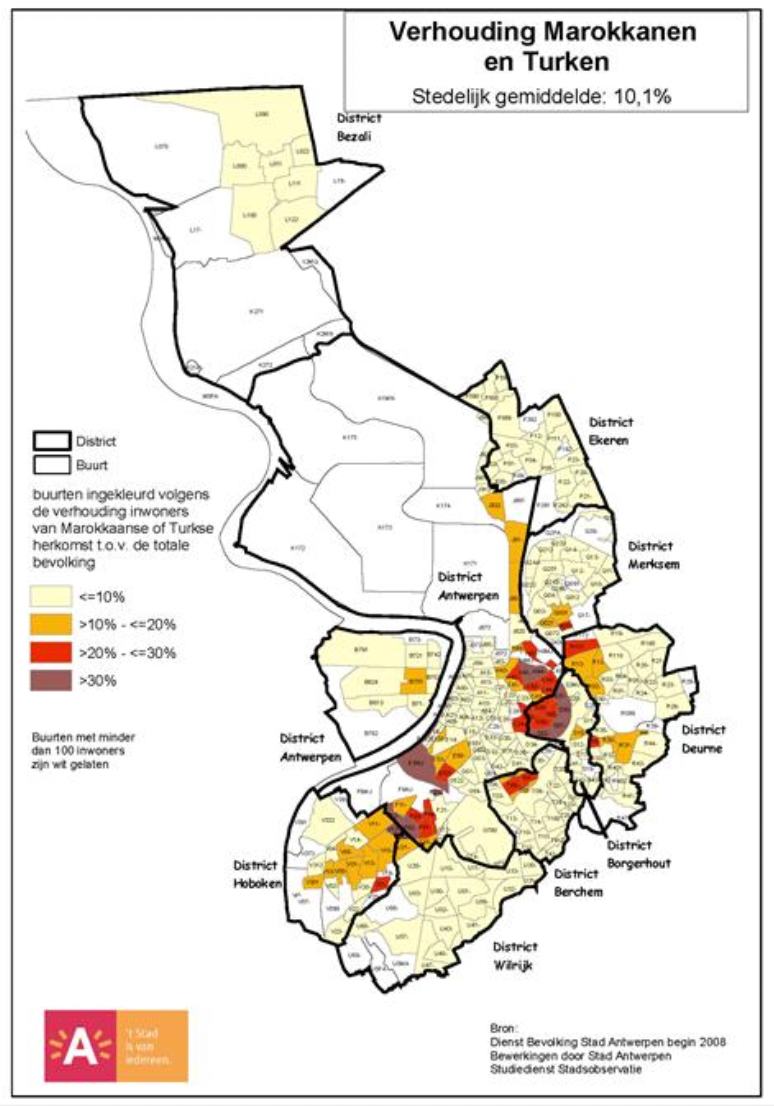
\includegraphics[width=20em]{examq_segregation_causes}\]

%%%%%%%%%%%%%%%%%%%%%%%%%%%%%%%%%%%%%%%%%%%%%%%%%%%%
%																	LECTURE 5
%%%%%%%%%%%%%%%%%%%%%%%%%%%%%%%%%%%%%%%%%%%%%%%%%%%%

\section{Neighbourhood effects and living with diversity}
\textit{November 8th, 2021 - Nick Schuermans}

\subsection{The ideal of social mix}

The ideal of mixed neighbourhoods has been on political agendas for a long time.
It is supposed that segregation has a negative effect on disadvantaged people (low-income, low-skilled), such that a disadvantaged person suffers more when living in a neighbourhood stricken by poverty, than in a neighbourhood without these ailments.

Different groups have different reasons for wanting social mixity: 

\begin{outline}
	\1 The \textbf{capitalist bourgeoisie} are afraid that the concentration of certain populations in a certain areas in a city, would have negative effects like revolutions, and that socialist thinking would become dominant
	\1 The \textbf{utopian socialists} were scared that the concentration of labourers would make it harder to create an egalitarian society
\end{outline}

The idea of social mixity is still dominant today and is high on the political agenda, worldwide, and across the whole political spectrum. Overall there are concerns about how the concentration of disadvantaged people and people of foreign origin affect \textbf{social mobility and cultural integration}.

\subsubsection{Examples of social mix}

\begin{outline}
	\1  Brussels Capital Region: ``Contrary to the American city, the ideal type for the European city is based on a mix of functions and people'' $\rightarrow$ ideal cities require a mix of people (poor, rich, local, foreign), and of type (residential, commercial, offices, etc.). The concentration of disadvantaged people in one area, makes it harder for these populations to be socially mobile, and they would be better off if they were living in a mixed income population
	\1 Ghent: attracting people with high-earning jobs will create a greater tax base, which will provide more capital to invest in the neighbourhood/city
	\1 Antwerp: regulation/efforts to prioritise a certain type of housing, ie. single family dwellings over smaller units, in order to attract more single families with higher income
	\1 UK: Housing Market Renewal (HMR), neighbourhoods mainly inhabited by disadvantaged people were plagued by demolition projects and construction of new dwellings. The idea is to transform the neighbourhoods, so that the inhabitants are no longer disadvantaged by it, and make it easier for people to climb out of poverty
	\1 USA\marginpar{cfr. Slater}: Cabrini Green in Chicago, many apartment blocks were torn down and new houses built, to attract a middle class in a neighbourhood previously inhabited exclusively by disadvantaged
	\1 South Africa: using social mix and spatial integration to increase socio-economic opportunities
\end{outline}

Given the vast attempts at social mix, we ask ourselves: \textbf{is it possible to create socially mixed neighbourhoods, and do we want to?}

\subsection{Is social mix feasible?}

Policies like HMR (Housing Market Renewal) actually end up shifting the poverty elsewhere spatially, and do not solve the issue at the core. A metaphor is the waterbed effect, the idea that ``moving chairs on the deck of the Titanic'' will only relocate the problem rather than fix it.

Gentrification comes with displacement, such that low-income, low-skilled people leave gentrified cities like Brussels, towards cheaper and more industrial, disinvested areas. Clusters of highly educated people converge towards Brussels, whereas cluster of low-income  concentrate in industrial/manufacturing areas such as Charleroi.
This illustrates the ``moving chairs on the Titanic'', where the disadvantaged are moved around within Belgium, but still exist, and their condition does not change. 

$\Rightarrow$ Thus, trying to create a social mix in some parts of the city (or country), displaces people and shifts poverty elsewhere, and ends up creating concentrations of poverty `down the street', eg. in Charleroi.

\textbf{Inclusionary housing/ zoning} in Cadix, Eilandje (Antwerp) is comprised of:
\begin{outline}
	\1 25\% social housing, including 15\% rent and 10\% buy
	\1 50\% ``affordable''
	\1 25\% ``residential''
\end{outline}

The mixes subsidised housing with non-subsidised. The city could have chosen to make more money by selling off the land to private developers, but chose to do otherwise, and impose a certain amount of social housing.

\textbf{So, is social mix feasible?} Yes, and projects that encourage social have integrated different populations, but it is hard to do in a situation where the market is dominant.

\subsection{Is social mix desirable?}

\subsubsection{Neighbourhood effects}

The assumption of neighbourhood effect is that ``where you live affects your life chances'' (Slater, 2013), and that ``impoverished neighbourhoods $[$could$]$ make their residents worse off'' (Friedrichs, 1998).

Different geographers have been asking different research questions (eg. ethnic cultural vs. socio-economic), and using different methods (qualitative vs. quantitative data, surveys), to understand neighbourhood effects.

Every study on neighbourhood effects bear birthmarks. It matters where a study takes place and studies need to be \textbf{provincialised and contextualised}.. 
Literature on the effects of segregation in the USA has been used to influence policy in Eastern Europe, but the context is different - for one, segregation in the USA is stronger than it is in Europe, where the welfare state is much more developed. When it comes to poverty, and the eradication of poverty, this contextual difference is important, and the ideologies can not always be transferred as-is. 

\subsubsection{Why it could matter where you live}

Seven arguments for why it could matter whether you are a disadvantaged person living in a disadvantaged neighbourhood, or in a mixed neighbourhood.

\begin{outline}
	\1 \textbf{Social network argument}: social capital is the connections between individuals, and the networks and norms of reciprocity and trustworthiness that arise from them
		\2 Argument: mixed neighbourhoods will create connections, such that poor people are better off
		\2 Mixing people creates \textbf{bonding capital} between socially homogeneous people, eg. intra-ethnic, and \textbf{bridging capital} between socially heterogeneous people, eg. inter-ethnic
		\2 But
			\3 Increased mobility leads to \textbf{human extensibility}, leads to more networks and bonds outside the neighbourhood, especially at work or through kinship
			\3 Parallel lives: will drawing white families to Molenbeek help the people currently living there? Such people already have a social network outside of the neighbourhood, with people with the same social class, education status, etc. Thus, the middle class attracted to the neighbourhood will create connections with people similar to them, outside. This defeats the purpose of bringing middle class in, in the first place
			\3 Risks disrupting strong ties and bonding capital. Residents living in disinvested parts of the city, fall back on each other, ie. use bonding capital. Creating a mixed neighbourhood, by attracting the middle class, will displace the bonding capital that exists
			
	\1 \textbf{Underclass argument}:
		\2 \textbf{Structuralists} claim that poverty exists because of structural forces in a declining economic base (eg. move from fordist to post-fordist society, leading to lack of employment)
		\2 \textbf{Culturalists} claim that poverty exists because of a culture of poverty, with attitudes and behaviours that keeps people in their poverty. The ghettos (ie. neighbourhoods with concentration of disadvantaged people), with unemployment, vice, crime, addiction, disfunction, exist because of the \textbf{socialisation effects} (peer group effects, lack of adult role models) and the physical infrastructure and \textbf{institutional networks} within the neighbourhood
		\2 But
			\3 Causality: neighbourhoods with high concentration of drug use are located in the disadvantaged neighbourhoods; is this due to an uneven policing of disadvantaged neighbourhoods?
			\3 Socialisation outside neighbourhood facilitated by the internet, and people can connect via distance to people and media
	
	\1 \textbf{Social cohesion argument}: living in a neighbourhood with a high concentration of foreign speakers, will not acquaint you with the new country's language and norms, and this will make it harder to climb the social ladder. $\Rightarrow$ Ethnic segregation and socioeconomic mobility arguments for creating social cohesion
		\2 But
			\3 Mobility: is the neighbourhood the only place that such people can acquaint themselves with a new culture? There are many domains: home, work, leisure activities, where social mixing can happen outside the neighbourhood
			\3 Importance of local culture: protective spaces exist to give people a safe place to be, especially when they just arrive

	\1 \textbf{Local services argument}: a presence of the middle class will attract services, like banks and ATMs, and prevent food deserts. Mixed neighbourhood will attract a diverse set of shops and services
		\2 But
			\3 More differentiation will also lead to a differentiated demand: as diversity of people and businesses increase, some might not find what they are looking for; businesses might cater only to the middle class, and not the disadvantaged or ethnic groups, and thus displace the shops that previously existed and catered to low-income
			\3 Specialised services in arrival neighbourhood: will specialised shops and services (Thai, African...) remain?
			\3 Ethnic entrepreneurship will be overshadowed

	\1 \textbf{Political argument}: mixed neighbourhoods will be higher on the political agenda, because middle class people are more listened to or have connections to politicians. 
		\2 But, why do politicians not listen to the low-income populations in the first place?

	\1 \textbf{Spatial mismatch argument}: 
		\2 Concentration and clustering: in which part of the city is poverty concentrated? There is a mismatch between the location where people live, and where they could work (ie. where low-skilled jobs are available). 
		\2 But,
			\3 Public transport tends to be better in Western Europe, giving greater spatial mobility
			\3 The language divide can make it difficult to get a job in your area, especially in Brussels which speaks three languages. Do you need a specific language competency?
	
	\1 \textbf{Stigmatisation argument}: Teachers, businesses, employers come into neighbourhoods with a stereotype/stigma, and will not give as good chances to the people living there than otherwise
\end{outline}

\subsection{What about the privileged?}
Some insights
\begin{outline}
	\1 Neighbourhood effects blames the poor for their condition, labels their livelihood as ``dysfunctional'' compared to that of the middle and upper classes
	\1 The segregation created by upper classes regarding schooling, transport, housing, are not seriously considered by policy makers. Until this structural limitation is realised, the conditions of lower classes will not change
	\1 Living in mixed neighbourhoods may sensitise the middle and upper classes on the socio-economic conditions of the lower classes
	\1 The house is built as an enclave, protected and safe from the lower class (eg. panic buttons, firearms, gated communities...)
	\1 The neighbourhood as an enclave, where rough sleepers are kicked out, woken up in the middle of the night and harassed until they leave
		\2 Economic privilege
		\2 Psychological privilege
	\1 A city of enclaves
\end{outline}


\subsection{Conclusion}

The concept of social mix is not very convincing. Gentrification simply moves disadvantaged populations to other parts of the city, which could be much worse, not provide the same services, and break social ties. 

When thinking about promoting social mix policies, we need need to ask:

\textbf{For whom?}
Why do we want to create a social mix? is it in the advantage of the underprivileged, or the privileged? for ethnic minorities, or majorities? for newcomers, or settled residents?

and, 

\textbf{Where and on what scale?}
The statistical units used to analyse segregation matters, are we looking at the city or regional scale? And where, only in disadvantaged neighbourhoods? only in gentrifiable, disadvantaged neighbourhoods? 
Why are we only concerned with disadvantaged neighbourhoods, and not other municipalities where we could ask whether it is worth creating diversity there.

and,

\textbf{Why?}
To counter poverty? To stimulate integration? There might be less costly, more effective policy alternatives than social mixing.
To counter racist stereotypes? To improve the local tax base? This uses the interest of poor people as rhetoric.

%%%%%%%%%%%%%%%%%%%%%%%%%%%%%%%%%%%%%%%%%%%%%%%%%%%%
%																	LECTURE 6
%%%%%%%%%%%%%%%%%%%%%%%%%%%%%%%%%%%%%%%%%%%%%%%%%%%%

\section{Cultures of Urban Research}
\textit{November 22nd 2021, Bas van Heur}

\textit{tldr; brief history of cultural theories, because history matters}

\subsection{Cultural turns in the humanities and social sciences}

Cultural turns are part of a wider shift since the late 1970s, in research practices in humanities and social sciences.

Why is there, or should there be, a cultural turn? There are various interrelated claims:

\begin{outline}
	\1 \textbf{Empirical}: culture is increasingly more important in advanced societies
	\1 \textbf{Theoretical}: need theories to better grasp cultural dimensions of the social like symbols, affect, meaning
	\1 \textbf{Methodological}: need new methods to better interpret empirical data, or to interpret new data differently
	\1 \textbf{Better, compared to what?} The culture turn ``does things better'', but better compared to what? We need cultural turn because we need better methods (compared to number crunching)
\end{outline}

In the late 1980s to 1990s, these claims were being made more forcefully.

\subsection{Postmodernism and the city}

Fredric Jameson, \textit{Postmodernism, or The Cultural Logic of Late Capitalism}, 1984. He is a Marxist literary and cultural theorist, writes about modernity and postmodernity, and relation of culture to the political economy\footnote{Political economy is a code word for capitalism}.

\textbf{Jameson's Postmodernism}

Postmodernism as the cultural logic of late capitalism:
\begin{outline}
	\1 Postmodernism is not a style but a cultural dominant
	\1 Commodification of culture: ``aesthetic production today has become integrated into commodity production generally''
	\1 Postmodernism as a \textbf{third stage of capitalism} (ref. Mandel): postindustrial, late, multinational, consumer capitalism as the political economy side of postmodernism. Postmodernism defined as such can only describe society after 1930s
\end{outline}

The Bonaventura Hotel is for Jameson the culmination of late capitalism. It aspires to be a ``total space, a complete world'', with hidden entrances and \textbf{separate from the city}\footnote{Think about other elements of the city that exist in the space, but are actually separate: gated communities, privatised public space,...}. It's impossible to navigate postmodern hyperspace and situate yourself in reality.

Constitutive features of the postmodern:
\begin{outline}
	\1 Superficiality instead of depth: textual play, beyond authenticity
	\1 Modern alienation of the subject is displaced by the postmodern fragmentation of the subject
	\1 Historicism effaces history; a recycling of the past, there is no linear trajectory
	\1 `Semi-autonomy' of the cultural sphere has been destroyed by late capitalism. But, not an extinction, rather an explosion: ``everything in our social life can be said to have become cultural''
\end{outline}

\subsection{Los Angeles School of Urbanism}

Jameson was influential for the cultural urban theories that came after him, such as the Los Angeles School of Urbanism.

The postmodern condition was a radically new urban condition, a \textbf{postmodern urbanism}. The main characteristics were:

\begin{outline}
	\1 It went beyond the Chicago School: urban fragmentation
	\1 LA and Southern California as privileged cases for research, and also considered LA as a prototypical type for the future cities across the world, specially on fragmentation and sprawl
	\1 Focus on restructuring: post-Fordism, flexible accumulation, late capitalism a la Jamesons
\end{outline}

Is the LA School really a school? It was soon critiqued internally and externally, there is not one single claim being made but rather a diversity within coherence (perhaps). The different lines of research:

\begin{outline}
	\1 Political economy: post-Fordism, flexible accumulation, industrial organisation, regional development
	\1 Homelessness, unskilled work, local labour markets
	\1 Political economy of place: element of the region, what does postmodernism mean for local labour and polarisation of labour markets
	\1 Environmental justice: transformation of the region has had effects on the environmental/ecology issues
\end{outline}

The LA school put LA on the map of urban studies. 

\subsubsection{Keno Capitalism}

Keno capitalism shows in the extreme how artists looked at postmodernism. It argues that the spatial manifestation of postmodern urbanism is `keno capitalism', making a reference to board game.

It represents a very fragmented form of urban structure. There is no centre that extends outwards or central planning, but rather, random developments throughout the city. It's almost a parody of the debate, and taken to the extreme and oversimplified.

However, cultural dimensions of Keno capitalism/postmodern urbanism resonate today:

\begin{outline}
	\1 Cultures of heteropolis: minority populations, urban diversity, cultural hybrids, ethnoburbs, Cosmopolis
	\1 City as a theme park: architectural dreamscapes, leisure simulacra with surveillance and control, spectacle, consumption
\end{outline}

\subsubsection{Critiques of the LA School}

Generally, you have to be respectful of what came before but this is not what the LA School did.

\textbf{What's new?} There is already existing work on diversity, restructuring, consumption and commodification, poverty.

\textbf{It's wrong to reduce the Chicago School to Burgess' concentric zone model}, as there was internal variety.

\textbf{There is an ethnographic void} in a lot of literature on postmodern urbanism. It relies on a detached, top-down interpretation of the city; marginalises agency and interpretation of `ordinary people', and there is no postmodernism from below.

\textbf{LA is not that radically different}. Existing urban theories are still relevant to explain what is happening in LA, and the empirical phenomena in LA are also visible elsewhere and were happening before or earlier than when the LA School discussed it.

\subsection{Urban landscapes and the symbolic economy}

Another strand of research that focuses on facts on the ground. It is completely different to the LA School, although developing in parallel.

Key guiding assumptions and arguments:

\begin{outline}
	\1 \textbf{Flexible accumulation and postmodernism} are two sides of the same coin, and are impossible to extract from one another; Marxist argument, similar to Jameson 1984
	\1 Rise of postmodernism goes along with the \textbf{rise of a new middle class}, with the rise of post-fordism, etc. that created a new type of labour and population that was highly educated, with well paying and intellectual jobs. They have new sensibilities and interests, and new lifestyle and consumption preferences
	\1 \textbf{Culture is key to urban redevelopment}: real estate, artists, representations of urban space. The impact of gentrification on city spaces, are artists encouraging gentrification or being kicked out of gentrified areas?
	\1 \textbf{Important role of the state}: the state investing in cultural landmarks, developing cultural and economic policies
\end{outline}

\subsubsection{Two sides of the same coin}

Paul Knox, \textit{The Restless Urban Landscape}, 1993: ``there is widespread agreement that the emergence of postmodern architecture, culture and philosophy in Western society has proceeded in tandem with the emergence of globalised, more flexible forms of capitalist enterprise''

\subsubsection{Rise of a new middle class}

Paul Knox, 1993:

\begin{outline}
	\1 Economic argument: emergence of new class factions under advanced capitalism; the hierarchy remains but different/new classes may become dominant
	\1 Sociocultural: generational reaction against modernist aesthetics, embracing instead postmodernism
	\1 Lifestyle orientation: self realisation/expression, cultural politics; positively, art becomes part of everyday life, or critically, art is just showing off your identity
	\1 Commodity aesthetics: niche consumption (eg. wearing certain shoes, listening to some genre of music, installing flooring in a house will change between people but a niche scale) with emphasis on taste and aesthetics, gives an increased role for design
\end{outline}

\subsubsection{Culture and urban redevelopment}

Sharon Zukin, \textit{Loft Living}, 1982. Focuses on New York City where there are lofts, but can be applied to a wider context.

\begin{outline}
	\1 The argument is that re-occupancy of abandoned structures by artists, followed by a new middle class (reconquest of the inner city), leads to a loft lifestyle which does not represent the typical architectural style (eg. single family suburban home)
	\1 Competing uses: there is a terrain of conflict between the remaining old tenants, the artists, and the middle class
	\1 When artists move in, it becomes more attractive for investors because the middle class may follow suit; hence, culture is used to develop and profit from emergent real estate market
	\1 Artists as drivers and victims of urban development
\end{outline}

Representation of urban space:

\begin{outline}
	\1 Role of media and marketing in putting cities on the map; urban images, what do we have in mind when we think about a certain city?
	\1 Contested (marketing) images
	\1 Urban tourism: European cities have always been key sites of tourism, first middle classes/aristocrats but has become more accessible since 1950s; Today airbnb

\subsubsection{Role of the State}

	\1 State strategies: originally business driven, but nowadays picked up by states
		\2 Cultural and economic policies: first strategies aimed at developing cultural industries, local economic development
		\2 Large-scale events: world fairs, art exhibitions attracting tourists and wealthy visitors
		\2 The arts and the urban growth machine: focuses on art/elite networks, using art institutions as local attractors for inward investment and urban development
\end{outline}

\subsection{Meeting halfway? Urban anthropology, cultural studies and the spatial turn}

The late 20th century urban geography was heavily influenced by the cultural turn, and related debates on postmodernism and globalisation. There was increased interest in ethnography, everyday life, imaginaries and representation.

The cultural turn intertwined with increased interest in spatial configurations and urban space in particular. Reasons include the post-1989 obsession with globalisation, and the critique of modernity (emphasising space and de-emphasising time).

There was increased interaction between urban geography, urban anthropology, and cultural studies. Disciplines with longstanding and core interest in everyday life and cultural phenomena.

Core themes in urban anthropology/cultural studies influencing the interdisciplinary urban studies are \textbf{informality and everyday life}.

\textbf{Informality} of (local) labour markets, precarious work, migration, legality, political governance and contestation. 

Informal work is selling things in Las Ramblas and living a precarious life through informal work. Informal/formal is different from illegitimate/legitimate. for example, household work is informal but may not be illegitimate, compared to drug trafficking which is informal and more often illegitimate. 
Related terms: unregistered economy, black market, non observed economy, undeclared work, shadow or hidden economy.

\textbf{Everyday life} is agency, community (building), resistance, consumption, identity, media and representation.
People are active, creative agents and not passive consumers. Focus on participant observation, extensive period of fieldwork to gain trust and inside knowledge of everyday practices.
The `everyday' is a trans-disciplinary concept, and you need to look at the disciplinary specifics to understand the concept in context. 

For urban studies, Henri Lefebvre sees the everyday as a sign of utopian possibility but colonised by the commodity form.

Michel de Certeau, \textit{The Practice of Everyday Life}, 1984

\subsection{Conclusion}

The cultural turn is understood as part of a wider shift in analytical sensibilities in the social sciences (theory, methods).

Urban geography is one strand of the debate in this cultural turn. It is heavily influenced by a Marxist interpretation of postmodernism, as \textbf{the cultural expression of late capitalism}.

Work on symbolic economy has shifted attention towards questions of representation, urban lifestyles and cultural production. 

Increasing rapprochement between urban geography, cultural studies and anthropology as part of the spatial turn.

Research on informality and everyday life, and related concerns, has enormously contributed to the development of a truly inter/trans-disciplinary urban studies.

%%%%%%%%%%%%%%%%%%%%%%%%%%%%%%%%%%%%%%%%%%%%%%%%%%%%
%																	LECTURE 7
%%%%%%%%%%%%%%%%%%%%%%%%%%%%%%%%%%%%%%%%%%%%%%%%%%%%

\section{Urban Cultures}
\textit{November 29th 2021, Bas van Heur}

Key coordinates of urban culture over the last 40 years: Fredric Jameson's definition of postmodernism, to the 1980s-early 1990s on postmodern urbanism and the LA School, to the symbolic economy.

This lecture's focus is research on urban culture, but focusing on actual cultural expressions approached from the angle of urban studies.

\subsection{Meeting halfway? The spatial turn}

A rapprochement between geography becoming a cultural discipline, but also culture becoming more spatial/geographical.
Increased interaction between urban geography, urban anthropology, and cultural studies.

Core themes in urban anthropology/cultural studies are \textbf{informality and everyday life}.

\subsection{Informality}

The informal economy, labour markets, precarious work, migration, legality, political governance and contestation.
Related terms: unregistered economy, black market, non-observed economy, undeclared work, shadow or hidden economy.

Keith Hart, \textit{Informal income opportunities and urban employment in Ghana}, 1973. He focused on:

\begin{outline}
	\1 There is employment beyond government, factories, large scale commerce. There is a whole world of work that we don't see or capture because we don't have the vocabulary to describe it
	\1 Makes the distinction between formal and informal, which come from the economy to describe the work that can be taxed. The type of work he describes in Africa is mostly untaxed and so, informal
	\1 Makes the distinction between illegitimate and legitimate. The informal work does contribute to the economy, but on a smaller scale. For example selling food on a market is informal but legitimate, but bribery and corruption is informal and illegitimate
\end{outline}

Naming concepts like informal/formal and illegitimate/legitimate is important to put them on the table as concepts that can be discussed (think of feminist studies and informal work in the home).

Informality is interesting because it is a concept that started in global South, but has been picked up increasingly to understand practices in the North. It transcends the global South/North divide, and is no Euro or Western-centric.

Research is mostly on 

\begin{outline}
	\1 Opportunities but also precarities created by unregulated economic activities
	\1 Gendered dimensions of informal work, on women working in the home and in markets
	\1 Transnational dimensions: informal labour markets are often transnational; migrants sending remittances home, migrants occupying informal labour markets. For example, migrants from north Africa who are legal/illegal/semi-legal trying to make a living on the streets of Barcelona by selling trinkets
\end{outline}

\subsection{Everyday life}

Dominant in 1980s-2000s, a buzz word to refer to agency, community (building), resistance, consumption, identity, media and representation.

Everyday life is concerned with lived experiences and meanings constructed by subjects in their own world. 
People are seen as active, creative agents rather than passive consumers.

Tradition of community studies and
\begin{outline}
	\1 Focus on participant observation and extensive period of fieldwork to gain trust and inside knowledge of everyday practices
	\1 History in Chicago School, with research on `self-contained' urban areas and on various topics (gangs, ethnic segregation, lifestyles, delinquency)
	\1 Applying `rural' concepts of classic community studies applied to urban settings, like family kinships, traditions and rituals
	\1 Key critiques are being too localist, assuming community as homogenous, sharing the same values
\end{outline}

Some trends are

\begin{outline}
	\1 Conflict theoretical approaches instead of cohesion theoretical approaches. Eg, looking at social interactions between people but not assuming cohesion theoretically, but conflict theoretically (moving from Durkheim perspective to a Marxist perspective)
	\1 Focus on network ties (local and trans-local), care and support in unequal and changing urban settings
	\1 Shifting symbolic boundaries between communities, because of communities being how they actually are (conflicting) rather than how they are assumed to be (cohesive)
	\1 Communities of choice and elective belonging (subcultures like the gay community, and gated communities)
\end{outline}

A truly trans-disciplinary concept, connecting cultural theory with philosophy, Marxism, ethnography, post-structuralism, sociology, aesthetics... but that doesn't mean it's used in the same way.

For urban studies, the eternal references are: Henri Lefebvre who sees the everyday as a site of utopian possibility but also colonised by the commodity form. More empirically minded researchers like Stuart Hall and Tony Jefferson's 

\subsubsection{Subcultures}

Hall, Jefferson, \textit{Resistance through Rituals: Youth subcultures in post-war Britain}, 1976. 

Subcultures are the everyday, symbolic opposition/resistance to a dominant social order. They are the resistance, style, social practices, subcultures, codes, encompassed by the urban youth, identity, gender blindness, feminism, etc.

\subsubsection{Practices of Everyday Life}

Michel de Certeau, \textit{Practices of Everyday Life}, 1984. 

More poetic and less political than British cultural studies, It focuses on tactics vs. strategies, influential in shaping the distinction between producers and (creative) consumers. How groups or individuals develop tactics to resist, avoid, intervene. Tactics are situated (local), defensive or opportunistic.

Top-down strategies vs. top-down tactics is too simplistic, but has shaped the idea that we have media cultures to shape things but as creative consumers who can change and creatively interpret things.

\subsection{Arts, activism, urban engagement}

There is an established tradition of aesthetic analysis of painting, music, theatre, etc. But, in urban studies, arts and culture are used primarily as sociological/political economic approach towards the arts and culture.

Three main urban researches on the arts: 

\begin{enumerate}
	\item Public art and site-specific art
	\item Artists and urban social movements
	\item Popular culture and urban politics
\end{enumerate}

\subsubsection{Public art and site-specific art}

Rosalyn Deutsche, \textit{Uneven development: public art in New York City}, 1996.

A critique of the instrumentalisation of public art, and the notion of `the public', by local governments and developers. The government usually has budget to spend on public art, but the result is usually not very interesting or nice. Public art is used as a legitimation device for uneven development. There are `pseudo-public spheres' or oppositional spheres, which have a massive influence on the role that arts  can play in the urban.

She says we can't assume that simply putting public art in a public square we automatically address the public. People may not engage or understand it. It only makes it public if you automatically engage with people (the public). 

And that art in a gallery can be public as long as it engages with the public. She critiques the distinction between public/private art, and that modern art moves out from the gallery and to the public, because public art can also be in a private space. 

$\Rightarrow$ We can have art in public space, but it needs to engage with the public in order to be public art.

A famous example: Richard Serra's \textit{Tilted Arc}, 1981. The steel plate is a public intervention, a piece that cannot be ignored. The way it has been received illustrates the problems with public art:

\begin{outline}
	\1 Conservatives complained that it blocked their way of passage
	\1 The artist assumed that the fact that people had to change their everyday practices (by changing their route) meant that they had to engage with the art
	\1 The problem is that it relied on a very narrow aesthetic reading: it ignored everyday, useful practices. The idea that the public creates a dialogue with a piece of art, is ignored, and the art was not engaging with the public in the constructive sense
\end{outline}

Krzysztof Wodiczko's \textit{The Homeless Vehicle Project}, 1988. A vehicle designed by the artist in consultation with homeless people, used as a practical tool for managing their everyday life, including washing/sleeping/storage (notably for what was collected). The object was exhibition in galleries, but also used by homeless people and `making visible' the effects of uneven urban development, on a wider group of urban users.

\subsubsection{Artists and urban social movements}

There is a longstanding tradition of artists engaging in social movements, but mostly outside of urban studies. 
Within urban studies, the debate has been mostly about the critique of the creative class and the creative industry policies, or neoliberal and entrepreneurial urbanism more widely.

Novy and Colomb, \textit{Struggling for the right to the (creative) city in Berlin and Hamburg}, 2013.
The urban social movements of the history of squatting and demonstrations against urban renewal politics, ie. urban counter-culture.

The artists and cultural workers have a privilege role because they have access to media networks and familiar with communication techniques. Thus, artists can frame and reframe social movements. 

\subsubsection{Popular culture and urban politics}

Back to the classical core of cultural studies. A focus on popular culture as/in everyday life, as questioning authority and as imagining political alternatives. It's about politics beyond governments and politicians, to `street politics', `informalisation of the state'.

A classic case is hip hop. It focuses on community orientation and urban localities (`the hood', ghetto) as classic urban themes. It is also relevant for studies on commodification and globalisation of cultural forms.

\subsubsection{Conclusion}

There are different aesthetic strategies that engage with the urban: spectacle, grassroots, social work, arousing dissensus. These are analytically distinct, but in practice this isn't so but is `messier'. For eg. an artistic practice can be both social work and spectacle.

\subsection{Cultural infrastructures and informal urbanism}

Recently attention has been paid to the infrastructural dimension of urban cultures.

Brian Larkin, \textit{Signal and Noise: Media, Infrastructure and Urban Culture in Nigeria}, 2008. An anthropological study on the cultural work of media technologies and their role in producing what we call urban Africa.

He flags a number of debates that are essential in research on infrastructure, and cultural infrastructure. It's a lot about the symbolic and representational logic of infrastructures. What do infrastructures mean, how are they represented, how are they/what do they envision?

He also speaks of the attempts of governments to govern and control these infrastructures, and the unexpected consequences of the infrastructural development. Just because planners have one goal for the infrastructure, it doesn't mean that they will actually be used as such. There are informal social practices and every day life around these infrastructures.

Eg. Piracy in Nigeria and how services of piracy distribution developed in Nigeria. Very informal, barely regulated, illegal/illegitimate. 

\begin{outline}
	\1
\end{outline}

\subsection{}

\begin{outline}
	\1
\end{outline}

\subsection{}

\begin{outline}
	\1
\end{outline}


%%%%%%%%%%%%%%%%%%%%%%%%%%%%%%%%%%%%%%%%%%%%%%%%%%%%
%																	LECTURE 8
%%%%%%%%%%%%%%%%%%%%%%%%%%%%%%%%%%%%%%%%%%%%%%%%%%%%

\section{Transport and Cities: a Historical Hegemony}
\textit{December 13th 2021, Wojciech Keblowski}

\subsection{Transport and urban form: from pre-industrial city to Fordist city}

Why is transport important in the city? 

\begin{outline}
	\1 Impacts urban form and spatial arrangements of the city: how the city is structured, typically around transport
	\1 Transport is part of the environmental impact of cities, is both a problem and a point to address
	\1 Use different opportunities the city provides: work opportunities, leisure
\end{outline}

Santiago de Chile protests: addressed fundamental structural issues on how capitalism develops in the country, but the start of the protest was the increase of public transport fare.

Brussels: public space protests against cars, claiming they take space from people and decrease the quality of urban life.

Stockholm: climate strikes showing the necessity of us to radically change our behaviour, fast.

Some solutions are offered by platform-based economies, shared/digitalised economies, gig economies. Living in the city of the future, we won't need a car - we can rent one through an app, use e-scooters, etc.

\subsubsection{Transport and Urban Form}

Urban transport systems are strongly and intricately related to urban form and spatial structure. Urban development is intricately linked with the evolution of transport technology - does the city shape transport, or does transport shape the city?

The development of city is shaped by development of transport (including walking, cycling, public transport, car).

\begin{outline}
	\1 \textbf{Pre-industrial city}: walking, other means of transport were expensive
		\2 No motorised transport modes, having a horse carriage costs a fortune and is a luxurious good. Everyone walks, and the city must be of a size that is walkable
		\2 Urban form: a city of 5km diameter, high mixity of uses and density (100-200 inhabitants/ha), grid street pattern except in medieval cities, little distinction between workplace and home
		\2 Inventions: steam and electric engines (end of 18th century) and bicycle (1860s) were initially luxurious goods and for pleasure before becoming a mode of transport for workers; led to the \textbf{mechanisation} of land transport systems. 
		
	\1 \textbf{Industrial city}: tramway
		\2 First public transport systems: horse-drawn carriages, then electric tramways, railroads, metro $\Rightarrow$ \hl{revolution in urban travel}
			\3 Horse drawn and electric street cars emerge in Europe in late 1800s and become extremely popular in early 1900s, led to a revolution in how the city could be conquered by its inhabitants
			\3 Underground systems: started in London in 1863, then Budapest in 1896, and Boston in 1897
			\3 Railway transport systems became dominant system for people and goods on land
			\3 \textbf{Increased operating speed = increased coverable distance}
		\2 \textbf{Change in urban form}
			\3 Breaking up the compact and dense form
			\3 Expanding city to suburbs, connecting city to villages, becomes possible; city walls are destroyed
			\3 Expansion of urban form allows for specialisation of economic functions; creation of working class, new diverse social group selling its time for a living
			\3 First separation between work and home: people commute

	\1 \textbf{Fordist city}: invention of the car and the massification (making luxury products available to masses) of private vehicles in the 1930s
		\2 Universalisation of Ford cars (no customisation, personalisation), Taylorism, reaching a near automated way of producing vehicles, meant that the final price could be reduced as much as possible $\rightarrow$ \textbf{massification and era of automobile}. From 1913-1927, Ford built 15 million vehicles making it 2nd most produced car after WW Beetle 
		\2 \textbf{Increased operating speeds and distances}
		\2 Mass increase of car ownership 1920-1960s
			\3 Profound transformation of levels of personal mobility
			\3 Profound impact on urban (transport) policy and planning
		\2 Major road-building urban and nation-wide programmes $\Rightarrow$ urban resistances and struggles
			\3 Examples of highway projects: FDR Drive (NYC), Ponte Morandi (Genoa), Ring Belge (Charleroi)
			\3 Different trajectories across global regions (eg. China vs. USA; in China the construction happened in a very short time, from 2006 onwards the demand for concrete was bigger in all other countries in the world combined, a boom of unprecedented scale)
		\2 Motorisation and suburbanisation:
			\3 Suburbs and rural areas become accessible and interesting for people to settle in: more space, more `freedom', close to nature, etc. This is not a trend anymore today
			\3 Increased separation between urban functions: residential, industrial, commercial, specialisation, mono-functionality, lower density
			\3 Spatial results: from grid pattern to curvilinear, cul-de-sac patterns; size of the city is greater than 100km; increased spatial imprint of transport infrastructure (<60\% of surface in US) 
		\2 Decline in public transport
			\3 Decline in North America and Europe: as car became more popular, people lived in suburbs, commuted to white collar jobs in the city, (private) public transport companies ran into financial difficulties, they were nationalised (in some countries especially Western Europe) but their societal road declined and were for the working class
			\3 New wave of urban planning strategies focusing on public transport corridors in suburbs

	\1\textbf{Post-Fordist city}: ICT, air
\end{outline}

\subsection{Neoclassical perspectives on urban transport}

Capitalist system shaped the development of the transport networks.

In France, the territory was split in departments based on a regular grid. The administrative reform in 1791 replaced feudal/tribal control of territories, but split in administrative departments. For this development, the State needed a universal and reliable system to measure space: time, space, quantity (meters), and the metric system was not in place and accepted by all until end of 17-18th century. Until then, the huge diversity and locality in how to measure time, space, and quantity varied across space.

With the metric system, the State was able to create socio-economic developments that we know today. This colonisation of space was crucial for the development of infrastructure (electricity, water, rail, etc.). 

Today, the \textbf{colonisation of space} is no longer a national matter, not only nation States developing this project, but happening on a global scale. A whole science developed around the colonisation of different measuring systems. 

\begin{outline}
	\1 Transport engineering and transport economies: a commanding neoclassical position embraced by academia and practicionners
	\1 `Neoclassic' economics: an analysis of the determination of goods, outputs and income distributions in markets through supply and demand; transport is a commodity offered in a market, passengers are the consumers
\end{outline}

Two general principles of neoclassical transport:

\begin{outline}
	\1 \textbf{1. Rationality of transport}
		\2 Transport is a highly technical, expert-led, top-down discipline, reduced to absolute universal measure, a science that cannot be opened to general debate; knowledge of transport is acquired from empirical data and not from theory; transport geography and economies are objective
		\2 The user is a rational being, a `homo-economicus', conducts everyday an analysis on what is the most efficient way to get to the destination, purely utilitarian travel choices
	\1 \textbf{Transport as motor of economic growth}
		\2 Improvement of transport infrastructure leads to higher speeds and lower travel times, which lead to lower transaction costs
		\2 Transport development creates urban economic development, and vice versa; this is debatable
		\2 Travel time is monetised and ``unproductive''; but cycling is a multi-faceted activity which is not purely moving between spaces, but can be leisure, exercise, meditation, etc. 
		\2 This way of thinking about transport leads to the key problem faced by transport planning and policy is \textbf{congestion} which engineers focus on. \hl{If you focus on the fluid flow of passengers and cars, any obstruction to this flow is an obstruction that needs to be solved; this obstacle needs to be solved because otherwise the system is irrational (1) and it hampers the economic growth (2)}
	\1 But, there isn't enough proof that these principles hold
\end{outline}

What happens when you believe that what you do is rational and important for society and the economy? You engage in developing increasingly more complicated mathematical models to understand what is happening, and what will happen. Modelling human behaviour to know where people will be going. 

The problem is that this approach is devoid of social, theoretical, political discussion. Homo-economicus depicted as a purely objective being, and the issues of age, gender, class, ethnicity, is not taken into account and are not given any importance. The exposure of anti-capitalist, Marxist, feminist etc. theories are absent in engineering studies.
Key concepts of neoclassical transport are \textbf{transport demand and supply}.

\textbf{Where is the city} in neoclassical transport? It is a field of application rather than a site or outcome of socio-economic political and spatial dynamics. For the model to be as efficient as possible, pre-industrial elements must be erased for the new model to be applied. The city is a playground for technical and rational solutions, and today transport development follows rational ideals: if there is congestion, the (planner's or engineer's) solution would be to add to the infrastructure because traffic jam generates lost time, and is a detriment to the economy. 

For example:

\begin{outline}
	\1 Mono-functional urban planning and separation of functions
	\1 Physical separation of people and traffic (foot bridges, sidewalks, to allow the cars to have smooth space and movement while pedestrians go out of their way)
\end{outline}

\subsection{Sustainable urban transport}

Oil Crisis of 1970s. In 1973, the organisation of Arab oil exporting countries, ie. the Persian gulf countries, created an embargo, and the Iranian revolution in 1979 which couldn't be predicted (geopolitics cannot be modelled) caused the oil prices skyrocketed.

Reflection on the environment and the impact of the car, and on sustainable urban development. Why is sustainability important?

\begin{outline}
	\1 Transport, locally, is the largest local source of pollution
	\1 Transport, globally, is the largest single source of global transport-related emissions, the fastest growing contributor to climate emissions
	\1 The increase of urban population means an increase in mobility levels
	\1 On a global scale, urban transport is predominantly and increasingly car-based; car sales are rising, especially of SUV since 2018-2019 whose CO2 emissions are larger than smaller vehicles
	\1 $\Rightarrow$ \hl{the global climate problems are increasingly transport problems}
\end{outline}
 
%%%%%%%%%%%%%%%%%%%%%%%%%%%%%%%%%%%%%%%%%%%%%%%%%%%%
%																	LECTURE 9
%%%%%%%%%%%%%%%%%%%%%%%%%%%%%%%%%%%%%%%%%%%%%%%%%%%%

\section{Critical Perspectives on Urban Transport}
\textit{December 21st 2021, Wojciech Kebłowski}

\subsection{Review of last class}

Transport (and general city) planning has a \textbf{double rationality}: rationality of the discipline, as a field deriving from national sciences, laws of physics, apparently help to understand how people move around the city; and the rationality of humans, users, who makes choices on where and how they go.

The car was judged as the best, most economical, rational mode of transport. However there were problems related to the massification of the car, mostly social and environmental. There is a lot of infrastructure that needs to be built to support the car.

\subsubsection{Post-Fordist city}

\begin{outline}
	\1 Since the 1970s, cities have entered a post-Fordist era. There was a rapid development of telecommunications and air transport, leading to a \textbf{globalisation of trade}
	\1 Shift from industrial to service economy
	\1 Suburbanisation of not only housing, but also office and retail function; this created polycentric, mosaic like urban configurations, ``suburban downtown'', ``edge cities'' are new constellations
	\1 The symbol of this transformation could be seen in the airport:
		\2 Originally a functional place, of arrival and departure
		\2 This has completely changed, eg. Schiphol airport. It is a place around which the city develop; the type of airport a city has dictates the type of investments, business, etc. the city has; it is a landmark of urban marketing and development; around Schiphol are other activities business districts, office spaces, residential, hotels,... it is a sort of neighbourhood that develops around the airport
	\1 Why is this important? The flexibilisation and fragmentation of production and labour is increasingly complex; labour is much flexible and irregular, which has repercussions on transport 
	\1 $\Rightarrow$ Dissolution of regular commuter patterns: eg. people working at night need transport then, there are new uses that did not exist before
	\1 $\Rightarrow$ Challenge to fixed public transport networks: the night transport is organised for people out for leisure, not for work (eg. getting to the airport early)
	\1 $\Rightarrow$ Increased motor vehicle use in cities
\end{outline}

\subsection{Deconstructing sustainable urban transport}

Main conceptual solution from Banister (2008) is \textbf{sustainable mobility paradigm}. It revolutionised urban transport mobility.
It is summarised as:

\begin{outline}
	\1 Assumption is that we need to break with mono-functionalism, and engage in planning cities that are much more mixed, where different functions are allocated closely to each other; this is required because it will reduce travel across the city, which has important repercussions on sustainability
	\1 Can facilitate shift from unsustainable transport and limit the domination of the car, towards public transport, collective mobility, and soft transport like walking and cycling
	\1 Thus making mixed cities and make other transport modes than cars more attractive. But how?
	\1 People make rational economic choices, and in some places the car makes sense. There are also behaviours and lifestyles, social forces of inclusion and exclusion, accessibility, citizen participation that determine how people travel
	\1 Where is the city in this sustainable mobility paradigm?
		\2 The city is an outcome: sustainable transport is an integral component of a good, liveable, vibrant, vital city (Jacobs 2011, Banister 2011). Sustainable transport is:
		\2 Economically performing: move away from the car and economies continue to thrive
		\2 Creates social cohesion and diversity
		\2 Environmentally friendly, healthy, participative... 
\end{outline}

Everyone wants to live in a city with the attributes above. What policies, projects and practices exist? A typology

\begin{outline}
	\1 Tackling automobility
		\2 Improving vehicle technology: cleaning the engine, make it less polluting, replacing diesel with electricity or biogas, changing the construction to cause less casualties $\rightarrow$ But the greatest increase in car sales recently are SUVs, the most dangerous cars for pedestrians and the most polluting
		\2 Restricting car accessibility: impose pricing instruments like congestion charges, reducing the capacity of urban arterial roads, creating car-free ``pedestrian'' zones and shared spaces
		\2 Increase of public transport quality and accessibility
			\3 Some best practices include BRT, urban trams, urban funiculars, etc.
			\3 BRT, Bus Rapid Transit: predominant in Latin America and South Africa, but also in global North, creating separate lanes only for buses which are supposed to make travel faster throughout the city. It imitates and replaces an underground system, which is very costly infrastructure
		\2  Promoting the notion of ``multi-modality'': creating options so that people can choose between the car and something else, where this something else has many options, so they can choose what fits their behaviour and lifestyle best
	\1 Reducing the need to travel
		\2 Promoting proximity and density: transport oriented development
		\2 ICT (telework, teleshopping), trip substitution, trip switching, shared transport
		\2 $\Rightarrow$ These are allegedly `radical' interventions, ``renewing'' cities and making them more sustainable, green, attractive (Reigner et al, 2013), giving them back to the people
\end{outline}

So what are the critical questions that geographers can ask?

\subsubsection{Key problems}

\begin{outline}
	\1 Domination of neoclassical and sustainable perspectives on urban transport
		\2 The term sustainability has been appropriated by the car and oil industries, with regards to their production; but the questions that cities ask about eh sustainable paradigm can only reveal sustainability to a point
		\2 A largely unproductive debate in academia and policy circles
\end{outline}

\subsubsection{Looking critically at urban transport}

\begin{outline}
	\1 \textbf{Technological determinism}: more attention given to technological solutions, rather than political and social innovations (eg. how to incentivise people to use public transport)
		\2 People use individual transport because it goes where you want, when you want; thus cars should be clean so people can continue using them; eg. Elon Musk, tesla, electric vehicles, creating parallel motorway systems underground in LA; the discussion here is to solve congestion, and not making transport more accessible
		
	\1 \textbf{An atomistic and moralising perspective}
		\2 Focus on pedagogics instead on politics (Reigner, 2016): we can convince people to change habits and lifestyle related to transport and mobility, and in this way solve a number of issues related to the field of planning and policies
		\2 This means that within the sustainable paradigm, policy makers and stakeholders would engage in the pedagogics around transport than on transport itself
		\2 $\Rightarrow$ Deeply revanchist moral geography, there are good (cyclist, pedestrians, city centre inhabitants) and bad (car users, urbanites)
		\2 $\Rightarrow$ What are the structural causes behind transport related behaviour? Policies, infrastructure, affordability (car subsidies, cheap parking...)
		
	\1 \textbf{Uneven geography}
		\2 Urban cores are ``saved'' from the car, compared to road infrastructure that continues to develop in urban peripheries
		\2 Walking, cycling, public transport are given prominent position on the surface, while highways and car parkings moved to the underground
		\2 Eg: car-free cities limiting or banning traffic and parking of types of motorised vehicles. The alleged goal is to limit air pollution, tackling congestion, improving public space thus boosting life quality
		\2 Eg: congestion charges
\end{outline}

Congestion charging and urban tolls

\begin{outline}
	\1 Came from Singapore in 1970s as a neoclassical tool of planning, traffic jams were a thing and so tolls would limit congestion; it entered the sustainable transport paradigm (aim is to raise revenue for public transport, to generate a modal shift, improve air quality); put in place across Europe
	\1 Gained a lot of attention, but there is questionable evidence of results: 
		\2 Decongesting traffic but transferring congestion elsewhere (Madrid, London)
		\2 Supporting public transport but are revenues reinvested in road infrastructure (Oslo for sure, London)
		\2 Improving air quality but limited evidence with very local impact (London, Milan)
	\1 Key urban problems and critiques:
		\2 Social segregation: 
			\3 Discrimination of socio-economically vulnerable users, whose car and toll may not be paid for by their company
			\3 Segregation of users according to their means, and the economic value of their commute (economic valorisation of movement)
			\3 $\Rightarrow$ \textbf{commodification} of transport systems and space, people don't pay according to their means but according to the price set by the market. Road infrastructure is a neoliberal serviceand not a common good
		

\end{outline}
Neoclassical: humans react to the market prices, and so adjusting the price (eg. tolls) will influence people's actions and have a desirable outcome

Eg. does Uber impact the presence of car? Uber collectivises the car but also causes more traffic in cities where it operates; not to mention working conditions, it becomes a question of ethics and labour practices too.

\subsection{Exploring critical approaches to transport and mobility}

\begin{outline}
	\1 
\end{outline}

\begin{outline}
	\1 
\end{outline}

%%%%%%%%%%%%%%%%%%%%%%%%%%%%%%%%%%%%%%%%%%%%%%%%%%%%
%																	SEMINARS
%%%%%%%%%%%%%%%%%%%%%%%%%%%%%%%%%%%%%%%%%%%%%%%%%%%%

\section{Seminars}

\subsection{Seminar 1: World/Global cities}
\textit{October 19th 2021, David Bassens}


\subsection{Seminar 2: Diverse Cities}
\textit{November 18th 2021, Nick Schuermans}

\subsubsection{Muster et. al, ``Socioeconomic...''}
\begin{outline}
	\1 Spatial segregation hypothesis:
		\2 
	\1 Discussion
		\2 Assumption that socio-economic segregation is a cause, not a symptom; implies that the problem is concentration of classes (ie. space), and the solution is social mix; 
		\2 Local context and time are important for understanding the socioeconomic segregation in a given place
		\2 Does not mention capitalism
	\1 Discussion questions
		\2 If you reduce spatial segregation will this reduce socio-economic inequality?
		\2 Why do researchers of urban social mixing/spatial segregation place an emphasis on diversifying the residential housing stock? Can you think of other urban spaces in which socio-spatial mixing can occur?
\end{outline}

\subsubsection{XXX, ``Paradoxes of (post-) socialist segregation: XXX''}
\begin{outline}
	\1 Cities were more segregated before WWII, than during socialism; 
	\1 Highly sensitive to historical context
		\2 Warsaw: in WWII city was destroyed and communities displaced; socialist focus was to reconstruct; socialist regime had patterns of meritocracy (higher position in state = better housing); high income polarity between highly educated, middle class, and others
	\1 In global cities, income polarity has increased but  decreasing social segregation and concentration; this is rooted in the pre-socialist past of these cities
		\2 You might expect global cities to be wealthier and thus less socio-economic inequality, but this is not the case; actually the opposite
	\1 Discussion questions
		\2 If there is an increase in income inequality, but decrease of segregation, what does this mean for the city?
		\2 Does this mean that less segregation is always a positive indicator in cities?
\end{outline}

\subsubsection{Shien and Xiao, ``Emerging divided cities in China: socioeconomic segregation in Shanghai, 2000-2010''}
\begin{outline}
	\1 Economic restructuring, neoliberalisation, globalisation changed role of household type and lifestyle
	\1 	Socio-economic segregation factors
		\2 Housing reforms: abolition of welfare housing system, privatisation, opening of housing markets (commodification) $\rightarrow$ increase in housing price, development of housing in the suburbs
		\2 Educational composition
	\1 Discussion questions
		\2 
\end{outline}


\subsubsection{Visser et. al, ``''}
\begin{outline}
	\1 How young people's experience of the neighbourhood important for understanding how the neighbourhood works as an entity?
		\2 Lived experiences affect socio-spatial behaviour and life paths of people 
		\2 Youths have a view that differs from hegemonic discourse; neighbourhood effect studies should avoid overly simplistic descriptions of youths in deprived neighbourhoods; this paper gives agency to youths 
		\2 Youths are aware of their neighbourhood features and insights could be useful for policy makers
	\1 Discussion questions
		\2 What should be the role of youths in the neighbourhood effect research?
		\2 How do we define good (decent) social networks?
\end{outline}

\subsubsection{Schuermans et. al, ``Geographies of whiteness and wealth: white, middle class discourses on segregation and social mix in Flanders, Belgium''}
\begin{outline}
	\1 Is the middle class ready and willing to assume the role that policy makers assign to them through their social mix strategies
\end{outline}


\subsection{Seminar 3: Cultural Cities}
\textit{December 9th 2021, Bas van Heur}


\subsection{Seminar 4: Urban Transport and Mobility}
\textit{December 16th 2021, W. Keblowski}

\subsubsection{Sustainability Transport developments in Delhi, Stockholm}

\begin{outline}
	\1 The concept of sustainability in transport emerged in the 20th century after the global North was developed (eg. Stockholm, Sweden). 
	\1 In Stockholm: 
		\2 1980 car was a human right
		\2 1990s rapid expansion of automobile society
		\2 2000s congestion tax, new by-pass roads funded by pax revenues - what about socio-economic difficulties, some people require the car but cannot pay the tax - this creates segregation
	\1 In Delhi:
		\2 2000s: India as a ``global automotive power'', boosting economy
		\2 2006-2008: Bus Rapid Transit (BRT) system constructed and opened, but in 2015 efficiency was questioned and the plan of BRT scrapped; now the lanes are used by cars
	\1 Banister: both places think about sustainability but have different needs 
	\1 Although the approaches to sustainability of these two cities are different, the middle-class is decisive in which transport policies are implemented. This is problematic because sustainability can leave cities/countries in the spotlight of shame because of unsustainability, but at the same time sustainability practices may be unfair/exclusionary
	\1 Discussion
		\2 BRT in Ottawa: new BRT was implemented, 1000 buses ran/hour, but was not sustainable (diesel bus engines) and derailed 3 times last month (end 2021); example of modernisation for the sake of it
		\2 BRT in San Salvador, Honduras: working well and well used, but shut down because it was ruled unconstitutional because it was restricting access for car drivers
		\2 Policies and priorities are often politicised: San Salvador example above, India scrapping the BRT but promoting the metro
		\2 Paper hints that the more modern a city, the better the conditions in the city are to provide sustainable transport
		\2 Sustainability is important but a luxury/privilege: why would you address burning forests when people need food/water now?
\end{outline}

\subsubsection{Sustainability Transport developments in Chicago}

\begin{outline}
	\1 Neoliberalisation of local governments causes city government to see transport as entrepreneurial
	\1 City governments end up prioritizing the needs of wealthy residents, tourists, businesspeople - eg. rapid airport line, circle line around the CBD where the targeted people already have options and are wealthy/don't take public transport anyway, 
\end{outline}

\subsubsection{Spanish High-Speed Rail}

\begin{outline}
	\1 Critical account of HSR (Spanish high-speed rail) through lens of Harvey's spatial fix
	\1 Spatial fix: capitalism's drive to resolve its inner crisis through outward expansion; capitalism spreading over territory and spreading its presence, in Spain in this case
		\2 Capital accumulation: generating surplus, and reinvesting this surplus
		\2 Over accumulation: reinvestment does not generate return, so there is a devaluation
		\2 Spatial fix
	\1 Spatial inequalities in HSR: development of HSR has increased peripheralisation, and consolidated growth of already growing regions
\end{outline}

\subsubsection{Transport Justice}

\begin{outline}
	\1 Free Transit Toronto: demarketise transport and take it out of capitalist 
	\1 BLM: SF protest at Bart station and managed to stop Bart for a day, to show how discriminatory the public rail can be
\end{outline}



%%%%%%%%%%%%%%%%%%%%%%%%%%%%%%%%%%%%%%%%%%%%%%%%%%%%
%																	READINGS
%%%%%%%%%%%%%%%%%%%%%%%%%%%%%%%%%%%%%%%%%%%%%%%%%%%%

\section{Readings}

\subsection{Urban Geographical Traditions}

\subsubsection{Jonas et al., \textit{Urban geography: A Critical Introduction}}

\begin{outline}
	\1
\end{outline}

\subsection{Theories of World-City Formation}

\subsubsection{Friedmann, \textit{The world city hypothesis}}

\begin{outline}
	\1 Industrial capitalism has shaped city-formation processes. The city was no longer interpreted as social ecology (ie. natural forces based on space and population dynamics), but a social product of industrial capitalism
	\1 How are cities (urbanisation processes) connected to the world economy (global economic forces)? \textit{urbanisation processes $\Rightarrow$ global economic forces}
	\1 Emphasis on the city as a spatially integrated economic and social system
	\1 Seven thesis on world-cities:
		\2 Structural changes of the city are decided by the integration of the city with the world economy, and labour is divided in the new spatial arrangement
			\3 Spatial division of labour: national, regional, sub-systems, metropolises. Cities carry out HQ, financial, economic articulation of other regions, or all of these functions
			\3 Structural changes: external factors that are economic (capital flows, markets, wages...)
		\2 Key cities are `base' nodes in spatial organisation and articulation of production and markets. This creates hierarchies, there are clear axes (America, Europe, Asia)
		\2 The role of world-cities is reflected in their production sectors and employemnt
			\3 A small number of rapidly expanding sectors: HQs, finance, transport, communication, advertising, accounting, insurance, legal. But also a lot of low-skilled, low-wage workers in manufacturing, services, hotels, tourism, entertainment $\rightarrow$ a dichotomy
		\2 World-cities concentration and accumulation international capital
		\2 World-cities are destinations for domestic and international migrants
			\3 Capitalist countries try to curb international immigration, or limit to high-skilled or required workers. The metropolis receives international migrants, whereas the semi-periphery receives inter-regional migrants
		\2 World-cities highlight capitalism's polarisation, both spatial and class polarisations
			\3 Spatial: global (gap in wealth, income and power between countries), regional (income gaps), metropolitan (spatial segregation in inner-city ghettos, squats, ethnic working class enclaves)
			\3 Class: income gaps between elites and low-skilled; large scale immigration; structural trends in jobs
		\2 World-cities generate social costs that exceed state's fiscal capacities
			\3 Rapid influx of poor migrants, requires social reproduction that state can't (or won't?) provide fast enough
			\3 Corporations get tax-cuts and subsidies, furthering inequalities
			\3 The poorest have to deal with the burden of capitalist accumulation
	\1 What is a world-city?
		\2 A city that is a major player on the world economic scale, and whose structure is largely influenced by industrial capitalism
		\2 Marked by spatial, social, economic inequalities, especially between elites (high-skilled) and low-skilled/wage workers (typically migrants)
		\2 World cities see a lot of domestic and international immigration, which capitalist countries try to limit. States usually can't keep up fiscally, and with infrastructure (social reproduction) to support migrants.
		On the other hand, corporations get tax-cuts and subsidies. The burden of capitalism falls on the poorest
\end{outline}

\subsubsection{Sassen, \textit{Locating cities on global circuits}}

\begin{outline}
	\1 Change from inter-state system, to a firms and markets influencing state policies and cross-border standards
	\1 National economies are integrated with global circuits
	\1 The new organisation of these cities entails both geographical dispersal and mobility, and a territorial concentration of resources. The dynamics of dispersal and concentration entail globalisation, and top-level management control
		\2 Agglomeration is good for business. Central functions for business are concentrated
		\2 At the same time, there is a globalisation of economic activity
	\1 Urban centres expand, but so too does poverty
	\1 The new geography merges the global and the national
		\2 Cities go from being the most powerful in their nation, to cross-border networks. There are many global cities making up the network
		\2 Cities become disconnected from their region
	\1 Cross-border capital flows can be used to indicate economic globalisation. There is a concentration of flows
	\1 The CBD is no longer the central economic unit of a city, due to communication technologies (including travel)
	\1 As firms grow, the city too grows, but this means that social reproduction (infrastructure) must grow as well
	\1 In global cities, finance is the leading sector and can be highly digitalised. Yes it is not dispersed but concentrated in global cities
		\2 Digitalisation would make it easy to geographically disperse economic activity, yet they are strengthening cities as central places of coordination for firms
	\1 $\rightarrow$ Economic globalisation and telecommunication innovations have made way for cross-border networks. Industries have dematerialised and digitalised, and regulations (both national and international) make it easier for the global economy to exist
		\2 What came first, cross-border networks or economic globalisation?
\end{outline}

\subsection{Polarisation in World/Global Cities}

\subsubsection{Hamnett, \textit{The changing social structure of global cities: Professionalisation, proletarianisation or polarisation}}

\begin{outline}
	\1 There are three trends studied: professionalisation, proletarianisation and polarisation. These concepts have shaped the social structure of global cities, and the paper aims to understand whether there is a dominant trend
	\1 \textbf{Professionalisation} refers to an increase in ``professionalised'' occupations, with an increase in professional, managerial and technical workers, some on high income. Professionalisation started as a result of changes in the industrial structure (from industrialisation to a post-industrialisation era starting in the 1970s).
	\1 \textbf{Proletarianisation} is the increase in de-skilled jobs, as a result of changing industrial structures (basically the opposite of professionalisation, as a result of industrial structure changes).
	\1 \textbf{Polarisation} is the growing gap between the top and bottom ends of the occupational and income distribution, where the middle in shrinking.
	\1 Society went from a pre-industrial (pre-1840s), to industrial (1840s) and \textbf{post-industrial society} (PIS, 1970s). 
		\2 It shifted from a society dominated by manufacturing employment, to one dominated by the service sector and drastic decrease in manufacturing employment. PIS could be expected to give rise to de-proletarianisation (decline in working class) due to machinery and innovation replacing manual labour. On the other hand, capitalism generates technical innovation that could replace high-skilled labour, which would increase proletarianisation.
		\2 Researching the class structure of PIS shows that there is an upwards shift towards professionalisation, and that society is biased towards high-skilled labour (top and middle classes) rather than low-skilled (bottom class). Children with working-class parents and grandparents are now likely to be graduates and work in professional careers
		\2 However, the growth of professionalisation, and thus of the professional and managerial class, has been accompanied by an increase in income inequality and precarious work $\rightarrow$ polarisation
 \end{outline}

\subsubsection{May et. al, \textit{Keeping London Working: global cities, the British state and London's new migration division of labour}}

\begin{outline}
	\1 Instead of focusing on professionalisation and jobs at the top end of the market, this paper focuses on the bottom end and specifically on the character and composition of the people who work there (mostly  foreign-born and migrant labour). 
	It explores how state welfare, labour market, and migration policies have changed the labour market and increased the low-skilled labour demand, which is disproportionally taken up by foreign-born workers and new migrants.
	\1 It criticises Hamnett's work, saying that it focuses too much on professionalisation rather than polarisation
	\1 Regarding the state welfare policies, it did not protect wages or working conditions. Instead, Conservative governments tried hard to secure a competitive economic advantage for Britain by labour market de-regulation and welfare restructuring. The British state actively tried to facilitate the recruitment of migrant labour, at the same time restricting people's welfare.
		\2 A significant proportion of the bottom of the labour force are migrants, working long and unsociable hours, for extremely low rates, without protection offered to native workers like the benefits system
	\1 Bottom-up initiatives, and places of faith have taken on the role of campaigning for worker's rights s
\end{outline}


\subsection{Urban segregation: patterns and causes}

\subsubsection{Pacione, \textit{Land Use in the City}, 2009}

\begin{outline}
	\1 Morphogenesis: the study of town-planning, and what causes the city to have the shape it does
		\2 Urban landscape can be divided in three elements: land use (the most susceptible to change), buildings (less susceptible to change because their use can change without the building changing), town plan (street layout, most resistant to change) (Conzen, 1960)
		\2 Town plan is the outcome to the visions and policies of individuals (eg. landowners) or agencies (eg. local planning dept) that have the power to change the urban landscape
		\2 Need to understand the background, motivations and actions of the major agents in the development of townscapes
	\1 Human ecology: stems from the Chicago school
		\2 ``Competition among land uses for space resulted in the invasion of the most desired parts of the city and eventually the succession of existing land uses by a more dominant activity''
		\2 ``Natural'' areas would evolve, based on class and ethnicity 
		\2 \textbf{Burgess' concentric zone} model is an ideal type, with known limitations (which is why applying it to other cities can be difficult)
		\2 Public redevelopment scheme and government policies (eg. social housing), and gentrification of the inner-city, challenge the value of model today
		\2 \textbf{Hoyt's sectors}: urban land use starts at the city centre, around which the sectors are organised. The sectors grow only outwards. Critique is that it only represents residential housing and does not take into account class or ethnicity
		\2 Burgess' model focuses on the demand side of housing, whereas Hoyt's model focuses on the supply-side mechanisms whereby middle class housing develops in the periphery. Both are extremely simplistic
		\2 \textbf{Harris and Ullman's multi-nuclei}: the location and growth of the multi nuclei are based on factors such as, activities require specialised facilities, similar activities group together, some activities repel each other, and some activities must locate elsewhere than where is most convenient because of eg., high rent prices
		\2 Modern models: Mann's model of typical UK city, Kearsley's modified Burgess model, Vance's urban realms model, White's model of 21st century city
	\1 Political economy: seeking interpretations of urban change that reveals the structural forces underlying the observed land-use patterns
		\2 Capitalist societies, based on capital accumulation, are designed in such a way as to facilitate the transfer of profits and maximise the opportunities for investment $\rightarrow$ circulation of capital (Harvey)
		\2 Circuits of capital:
			\3 Primary circuit: the production process; surplus created during production is reinvested in primary circuit, or if there is not enough demand to produce more, in to the secondary and tertiary circuits
			\3 Secondary circuit: investment in fixed capital (built environment, real estate); profit is in the form of rent, or increased exchange value (sale price) 
			\3 Tertiary investment: in science and technology, ie. innovations to improve productivity, or labour capability (eg. health, education); this investment is usually made by the state
		\2 Contradiction between capital accumulation (provokes urban change and redevelopment) and the built environment (resists change)
\end{outline}

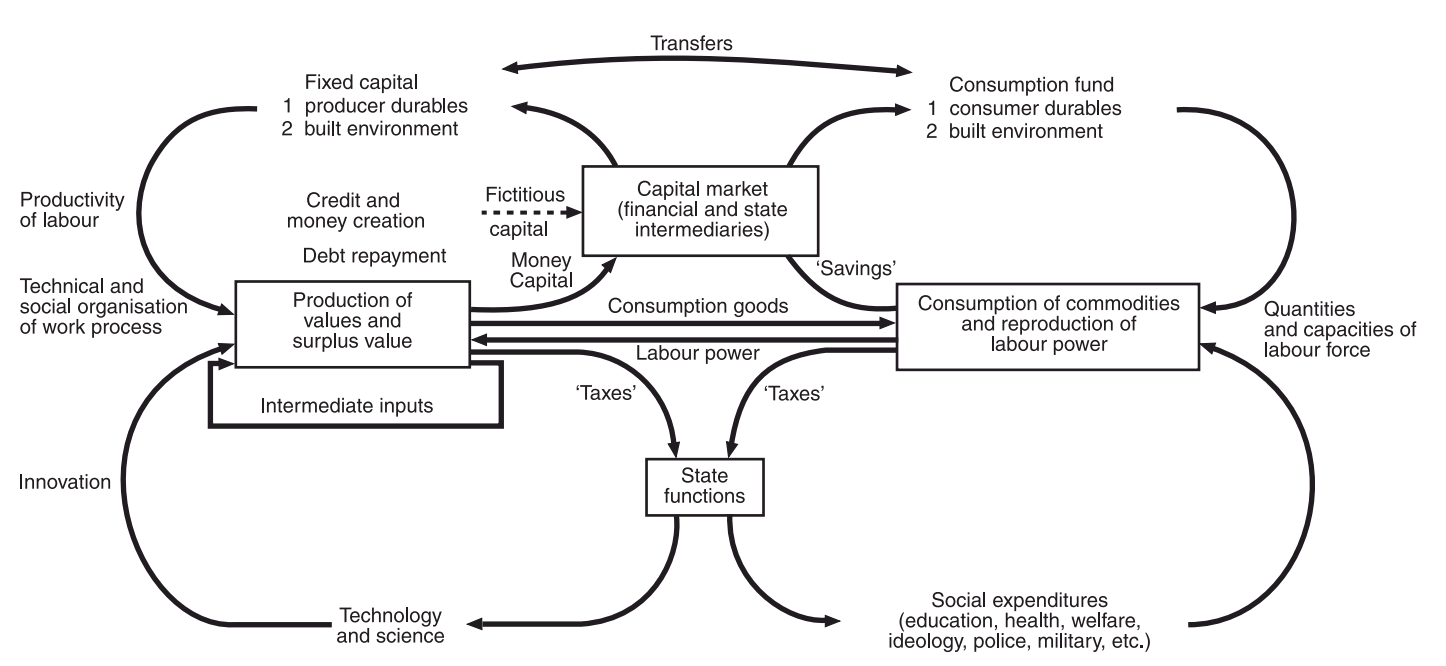
\includegraphics[width=\textwidth]{harvey_circulation_capital}

\subsubsection{Van Kempen, Sule Özüekren, \textit{Ethnic segregation in cities: new forms and explanations in a dynamic world}, 1998}

\begin{outline}
	\1 Segregation and concentration: \textbf{spatial segregation} is the residential separation of groups, ie. the degree of deviation from the uniform spatial distribution of all populations within a city. Spatial segregation implies \textbf{spatial concentration}, whereby one population group is disproportionately represented in a given space, compared to other groups
		
	\1 Disadvantages of spatial segregation and concentration
		\2 Living in a segregated/poor neighbourhood limits your opportunities in life (education, employment, health...)
		\2 Poverty has an effect on facilities (commercial and not)
		\2 Neighbourhood effects: the way the neighbourhood is viewed by others, and its stereotypes, contribute to self-fulfilling prophesies; this is a limited understanding, and is dangerous because it can lead to a lack of empathy towards those populations
		\2 Ghettos are ``institutionalised'': residents did not choose it for themselves, rather, they were coerced by society; residence is involuntary
		\2 \textbf{Underclass} ``suffer from prolonged labour-market marginality and have virtually no chance to alter this situation''. They're economically and politically isolated, usually have deviant or illegal behaviours, their lifestyle is one of survival and is different from that of the poor. Dangerous because it lumps together different populations, and normalises them
		
	\1 Advantages of spatial segregation and concentration
		\2 Existence and maintenance of social contacts is made possible by the concentration of like-minded people; it encourages cultures and norms that are not those of the mainstream society
		\2 Social networks allow people to support each other
	\1 Behavioural approach: explanations that include the preferences, perceptions and decision-making of the individual in housing and residential mobility
	\1 Ethnic-cultural approach: cultural differences between groups can help explain differences in housing conditions and residential patterns

\end{outline}

\subsection{Neighbourhood Effects and Living with Diversity}

\subsubsection{Van Kempen, \textit{Social consequences of residential segregation and mixed neighbourhoods}}

\begin{outline}
	\1 Investigates the social consequences of residential segregation of income and ethnic groups
		\2 ``How, for example, does living in neighbourhoods of poverty or ethnically homogeneous neighbourhoods have implications for education and the educational life trajectory of children? ... labour market careers?'' (p. 439)
	\1 In Western Europe, there is not much evidence that the neighbourhood affects the social conditions of its residents
	\1 Many authors say that the absence of a middle class, reinforce to poor social conditions of the low/working-classes, who end up living in a ``ghetto'', usually defined as a ```racial' or ethnic concentration of poor households'' (p. 440)
		\2 Reasons given are that ghetto residents don't see job opportunities and resolve to crime and ``anti-social behaviours''; they suffer from stigmatisation and discrimination
	\1 If poor residents suffer due to their residential concentration in some neighbourhoods, then there must be something that can be done to break the patterns of socio-economic segregation $\rightarrow$ enter social mix and ``balanced communities''
	\1 European ``ghettos'' look very different from American ones: the streets are cleaner, the buildings are in better condition, the reality of working class in Europe is relatively better than for the American because of a better welfare state
	\1 Policy makers seldom make decisions based on evidence
		\2 Provides examples of research showing the spectrum of relevance of neighbourhood with regards to socio-economic conditions
		\2 Describes approaches the policy makers take
	\1 Mixed-neighbourhood pros:
		\2 Opportunity for a housing career: the middle class who would have moved to a different part of the city, considers staying in the neighbourhood
		\2 Reconstruction of buildings is good when the buildings are in bad condition (still rebuilding affordable homes would be better but this doesn't happen)
		\2 When there is a large-scale vacancy it makes sense to demolish
		\2 After demolition and housing diversification, residents show more satisfaction and are less likely to move out of the neighbourhood
	\1 Mixed-neighbourhood arguments are problematic
		\2 No evidence that it helps lower-classes with regards to their socio-economic situation
		\2 Can force people to move in/out of a neighbourhood they did not want, demolition (to build middle class dwellings in its place) increases waiting lists for affordable housing, can decrease social cohesion and increase inequalities within the neighbourhood
		\2 Unmixed neighbourhoods have less opportunities for ethnic populations to exchange with `natives', but perhaps the ethnic population chose to be concentrated? 
		\2 Can social mix really fix wider issues like ``social polarisation, more cohesion, and high social mobility'' (p. 454)?
		\2 There is not enough empirical evidence, maybe because more time needs to pass before accurate research can be done, to judge the effect of social mix 
	\1 Concentrations of ethnic and socio-economic neighbourhoods are not all negative
	\1 Conclusion: not much evidence, especially in Europe, that unmixed neighbourhoods are worse than mixed neighbourhoods in socio-economic terms. Nonetheless it is popular amongst policy makers to want mixed/balanced neighbourhoods. Still, there are some good in mixed neighbourhoods, but bad when they are expected to have a positive effect on socio-economic conditions of the low-classes
\end{outline}

\subsubsection{Slater, \textit{Your life chances affect where you live: a critique of the `cottage industry' of neighbourhood effects research}}

\begin{outline}
	\1 The neighbourhood mix argument misses the point of why people live where they do. There are structural factors that put people in certain socio-economic conditions and that produce inequalities. It should be reframed as ``your life chances affect where you live'', which then addresses the \hl{problem of capital accumulation and class struggle}\marginpar{Finally someone saying this!}. Poverty is the problem, and moving people to a new neighbourhoods without addressing the systemic features of capitalism that create poverty in the first place, will not fix the problem
	\1 English mansions in Surrey, England, vs. Tower Hamlet blocks, a borough classified as ``multiply deprived'' for decades
	\1 Moving to Opportunity (MTO) vouchers randomly distributed to poor households, to move to low-poverty neighbourhoods
	\1 Uses Engels writing on industrial proletariat, which explains what shapes people's life changes; uses Marxist critiques of neoliberal urban land theory; critiques neighbourhood effect theories and policies that ignore the structural and institutional ``arrangements'' that create poverty and inequality; focuses on the stigmatisation of poor neighbourhoods
\end{outline}

\subsection{Cultures of urban research}

\subsubsection{Barnes, \textit{The 90s show: culture leaves the farm and hits the streets}, 2013}

\begin{outline}
	\1 Urban studies originally described the city as a place devoid of culture, and in purely economic terms (work, production, economic activity, Marxist, rent gap, urban gatekeepers, uneven development). Culture entered the urban studies sphere in 1990s, when cultural studies, postmodernism, new cultural geography emerged
	\1 ``My intention is to examine the processes by which culture came into urban geography, and the particular forms it has taken'' (p. 480)
	\1 Histories of urban and cultural geography, and their relationship
		\2 Sauerian (Sauer) cultural geography: focused only on the rural as a place of culture; extensive field research with natives; the cultural landscape is more than the sum of its parts, taking a holistic view of the cultural landscape, implies that there is an `environmental determinism'; emphasis local cultural and was skeptical of metropolitan power;
		\2 Beginning of urban geography in mid-1950s: was the anti-thesis of Sauerian cultural geography; believed in modernity, analysis, model and system building, quantitative empirical methods; urban geography was a spatial science
			\3 Urban geographers wanted to analyse the effect of modernity in the city
			\3 Analysis was a key tool: breaking down problem into quantifiable subelements, that can be related to each other
			\3 ``Radical political economists'' like Harvey and Castells put the city at the heart of capitalism. This ignores all cultural elements
			\3 Saurian cultural geography lacked a political purpose (Engels' accounts of Manchester, Marx' Communist Manifesto)
	
	\1 Reconciliation between urban and cultural geography, stemming from debates in political economy, cultural studies, and reconceptualisation of cultural geography
		\2 Cultural cannot be ignored when studying the city; it was ignored by urban geographers (either spatial or radical geographers) notably because of the connotations of Sauer and cultural geography
		\2 Revamping of urban geography by culture:
			\3 Outside urban geography emerged cultural studies and postmodernism that theorised the relationship between culture and economy
			\3 New cultural geography emerges, and critiques and replaces Sauerian cultural geography; says that culture is everywhere, from the most mundane to the most spectacular
		\2 Cultural studies showed that one could analyse class and the economy, while still recognising values, ways of life, and emotional and political commitments outside the economy
		\2 There are many discussions and positions on postmodernism
		
	\1 Specific forms that the ``cultural turn'' is taking in urban geography
		\2 In 1990s, urban geography increasingly became urban cultural geography; there was a merging of culture and economy, and urban geography became both, not either/or
		\2 Public space\footnote{Harvey, 1989, Conditions of Postmodernity} has become increasingly commodified, culture is used to extract money
		\2 Urban cultural industries: located in the worlds most powerful metropolitan centres. The economy is defined by new cultural products, and cultural products are produced because they are economic commodities.
		\2 Gentrification: originally in the 1980s either an economic argument, the rent gap theory (Smith), or a cultural argument, the postindustrial middle class making lifestyle and consumption choices (Ley); now, it is about both
		\2 Economic services and innovation: economy and culture are intertwined, capitalism is taking a cultural turn as businesses focus on ``creation, fostering and distribution of knowledge''; this happens in the city because that is where the forces exist that allow culture to be inextricably linked with the economy
		\2 International immigration and transnationalism: both economic and cultural factors, and class, gender, ethnicity, influence what patterns, changes, and resistance exist with regards to migration
\end{outline}

\subsubsection{Fredric Jameson, \textit{Postmodernism, or The Cultural Logic of Late Capitalism}, 1991}

\textit{Keywords: postmodernism, high modernism}

\begin{outline}
	\1 Architecture is the place where postmodernity emerged and is most visible
	\1 ``Every position on postmodernism in culture - whether apologia or stimatisation - is also at one ant he same time, and necessarily, an implicitly or explicitly political stance on the nature of multinational capitalism today'' (p.55)
	\1
\end{outline}

\subsection{Urban Cultures}

\subsubsection{Deutsche, \textit{Uneven development: public art in New York City}, 1996}

\begin{outline}
	\1 
\end{outline}

\subsubsection{Larkin, \textit{Signal and Noise: Media, Infrastructure, and Urban Culture in Nigeria}, 2008}

\begin{outline}
	\1 In Nigeria, infrastructure is not important in the sense that it provides resources (water, electricity) to people, but because it is a way for politicians to abuse their power by awarding contracts and obtaining political allegiance $\rightarrow$ \textbf{developmentalist ambitions of nationalism}
	\1 ``In the disaggregation from networked electricity to autonomous generators lies in the shift in Nigerian society from the developmental state to new forms of individual, competitive, liberalism'' (p. 244)
	\1 Infrastructure in colonial and post-colonial context
		\2 Colonial powers used infrastructure as a mode of rule, to show superiority, expertise in science and technology
		\2 On the other hand, Nigerians who could master the knowledge behind the infrastructure could take control over it 
		\2 Infrastructure reminds everyone of the government's failed promises, and is a way for the state to keep a tie between residents and itself
	\1 Infrastructure is a feature of Nigerian urban life: it works, it doesn't, it is shut off, the commodity (energy in form of electricity/gasoline, water) often runs out at the gas pump and is traded on the black market. This shapes urban life, what people can(not) do, how they respond (by having generators, using baths for water storage)
	\1 Because the State and infrastructure are unreliable, people turn to other networks (each other, religion)
	\1 Idea of the sublime: something that we are in awe of, that we surrender to (to some extent), such as colonial infrastructure. The sublime has to be redeployed as what was once sublime, is understood and becomes ordinary
	\1 tldr; infrastructure is technical, political and conceptual. People in Nigeria know how to operate outside the public infrastructure (eg. network grid) and are self standing $\rightarrow$ \textbf{individualism, competitive, liberalism}
\end{outline}

\subsection{Transport and cities: a historical hegemony}

\subsubsection{Banister, \textit{Cities, mobility and climate change}, 2011}

\begin{outline}
	\1 There are huge benefits of transport: globalisation of economies, better ICTs lowered the cost of transport
	\1 However transport contributes to CO2 emissions, and it is a sector where reducing emissions is difficult. At the same time it must play a role in reaching sustainability targets (emission levels)
	\1 Policies to reduce transport emissions include: reducing the need to travel, increasing access and use of public transport including walking and cycling, reducing travel distances
	\1 The reality in the EU
		\2 Although the causes of climate change are widely accepted, there is reluctance and lagging in behavioural change; the measures taken by the government do not match the urgency of the situation
	\1 Global perspective
		\2 The US has only 5\% of the world population, but 30\% of cars and produces 45\% of the world's CO2 emissions
		\2 Cities have taken on more responsibilities than nations in addressing transport emissions but ``there is considerable variation between cities'' (p. 1539)
		\2 Inequalities within and between cities: firstly, access to transport is not uniform and some cities have better access (are more equal) than others (eg. Beijing is `the most equal city in Asia' but Hong Kong has a lot of inequality). Second, most investments in transport infrastructure and services benefit the rich and not the poor (eg. India is going through an inequality trend similar to China following globalisation and liberalisation)
	\1 Mega-cities and sustainable transport
		\2 Cities with more than 10 million inhabitants. The growth of the population far outgrows the developments in infrastructure and services that will never be able to match the demand
		\2 ``These cities have tremendous potential for growth and will be the powerhouses of the world economy over the next decades, but they are also centres for potential unrest, as there is substantial inequality and poverty''
		\2 There is extensive urban sprawl, increasing distances between where people live/work/play, mega-cities are polycentric urban agglomerations, absorbing smaller cities in the process
		\2 Difference between high and low income cities: wealthy cities have the opportunities to invest in clean infrastructure, but poorer cities have more pressing social needs (although opportunities for environmentally sustainable policies exist)
		\2 Strong governance is required: the city must take responsibility and be the driver of sustainable policies, develop and implement them effectively, give a direction, and all stakeholders need to be involved in city-planning; the alternative will create unequal, sprawling, divided cities that are inefficient and unsustainable 
		\2 The mega-cities emerging are not new models of sustainable cities, but rather copies of car-centric Western cities
	\1 Clean planning strategies: mixed use developments, prioritise public transport developments (accessible corridors, near locations where locations are higher)
		\2 Plan the city such that walking and cycling distances are encouraged and the need for cars minimised\marginpar{But is this North-centric?}
		\2 ``cities would be designed at the personal scale to allow both high quality accessibility and high quality environment'' (p. 1541)
		\2 ``The intention is not to prohibit the use of the car as this would be both difficult to achieve and it would be seen as being against the notions of freedom and choice. The intention is to design cities of such quality and at a suitable scale that people would not need to have a car'' (p. 1541)
	\1 A street is not purely a road but can have other uses: a space for people and green transport
	\1 Planning for city futures: interrelationship between travel, urban form and sustainable development is complex
\end{outline}

\subsubsection{Reigner, \textit{Safe, sustainable... but depoliticised and uneven - A critical view of urban transport policies in France}}

\begin{outline}
	\1
\end{outline}

\subsection{Critical Perspectives on Urban Transport}

\subsubsection{Susan Hanson, \textit{Gender and mobility: new approaches for informing sustainability}, 2010}

\begin{outline}
	\1 Frances Willard, founder of the WCTU (Women's Christian Temperance Union) on learning how to ride a bike at 53
		\2 The bike (ie. mobility) went hand in hand with feminism; it would allow women to move around and would also change the expectation on their wardrobe, from something aesthetic to something practical
		 \2 ``Willard sees the bicycle as far more than just a means to regain her lost mobility after too many years of being trapped in decorous middle-class womanhood''
		\2 It brought her a sense of confidence and accomplishment
	\1 How does gender shape mobility and how does mobility shape gender?
	\1 Definitions
		\2 Mobility is ``personal travel that is part of people's participating in the daily round of activities such as paid and unpaid work''
		\2 Sustainable mobility should designed at different spatial scales, must be specific and use ``knowledge and practices in particular places at particular times''
		\2 Mobility isn't only about the individual, but about their embeddedness and interactions with society (household, family, community, society).  To think about mobility, one needs to consider the wider social, cultural and geographical context
		\2 Gender is the \textit{perceived} difference between men and women (and other genders) and the unequal power relations between them
	\1 How does mobility shape gender?
		\2 Woman mobility is equated to the home, domestic and private spaces, is routing and familiar, whereas men's mobility is equated to the urban, expansive movement, public spaces, new experiences, challenges
	\1 How does gender shape mobility?
		\2 Patterns of gender uses in mobility: when do women/men use transport, how far do they commute for work, what times of the day, does this change based on ethnicity
		\2 Causes of gender on mobility: fear of violence, power dynamics in the household, women not leaving their ethnic neighbourhoods (eg. because forbidden by husbands), post-migration experience shaping travel patterns of migrants
	\1 To provide sustainable mobility for women, you must understand the level of \textbf{agency} women have to take transport. When, where and how much is their mobility a result of \textbf{choice or constraint}?
\end{outline}

\subsubsection{Sheller, Urry, \textit{The new mobilities paradigm}, 2005}

\begin{outline}
	\1 Cosmopolitan taste from the North expects goods from around the world to be air-freighted to them, vs. people from the global South who use small scale import mechanisms
	\1 Social science, including sociology and urban studies, have tended to be static and ignored the automobile, or other technologies, which have had a significant influence on the development of society, culture, power relations, etc. and on people's mobility
	\1 Mobility is the transportation of people but also the communication of messages
		\2 Communication technologies (fax, phone, computers, etc.) have enabled one/many to one/many connections
		\2 Mobile/immobile infrastructures
	\1 Moving in space physically or virtually can be a show of status or power; ``there is the proliferation of places, technologies, and `gates' that enhance the mobilities of some while reinforcing the immobilities of others, including those of children'' (p. 213), also of women, marginalised groups, etc.
	\1 ``the greater the proliferation of such `tools' [cars, taxis, supporting services like customer service, email and phone contacts] and hence the greater the networking possible, so the more that access to such tools is obligatory in order to participate fully in a `networked society'''
	\1 New mobilities paradigm addresses the fact that activities are carried out while on the move, and that places travelled to are fixed and pull or push away people. Rather, places are not fixed but interconnected with nodes in the network of people, buildings, hosts, activities, transport, etc.
	\1 Six bodies of theory for mobilities research:
		\2 Simmel, science and technology research, spatial turn in social sciences,...
	\1 New mobilities: dematerialising connections, making and remaking networks with higher speeds; social networks built on top of technologies and platforms increasingly play a role 
	\1 Basically, new technologies including the ones in our pockets and the internet and the instantaneous exchange of information means that the world is increasingly more complex and everything is so interrelated that we need a new way of thinking about mobility, that takes into account more factors than the simple movement of people - but also of ideas, information, the virtual travel of these objects, the social relations, etc.		
\end{outline}

\subsubsection{Reignier, \textit{Safe, sustainable... but depoliticised and uneven - a critical view of urban transport policies in France}, 2019}

\begin{outline}
	\1 Public policies are not rational and do not address public problems, but rather are used to push an agenda, are ``vehicles for narratives'' (p. 220)
	\1 In France, sustainable mobility policies
		\2 are used to govern homo economicus, who is the nearly exclusive target of all public policies
		\2 are used to legitimise the upgrading of certain areas, ie. gentrification and inequalities in accessibility 
	\1 Mobility policies have been subjected to global competition paradigms, there is only room for rationality (in the policies and in people, ie. homo economicus). When people are nothing but economic actors, it `deactivates democracy' 
		\2 ``For Brown, this neoliberal rationality stimulates a process of deactivation of democracy when the citizens are nothing more than ``rational economic actors in every sphere of life'', when ``citizenship, reduced to self-care, is divested of any orientation toward the common'''' (p. 221)
		\2 $\rightarrow$ policies are favouring the economic rationality of individuals
	\1 Sustainability, health, safety have been used as three reasons to justify transport policies: to improve air quality, promote active mobility including soft modes of transport that are not ``aggressive for the city, for the urban landscape, or for the environment'', ie. pollution-free transport.
		\2 Depoliticising sustainable mobility by imploring moral and noble reasons: ``Legitimised by the mention of noble causes such as preserving an acceptable environment for future generations as well as people's safety and health, these narratives are presented naturally as being obvious, imposing the right way of doing things, the right way of behaving. The use of moral injunctions by the promoters of these public policies contributes to a process of depoliticisation'' (p. 223)
	\1 Fragile challenges in the face of moralisation
		\2 Costly and dubious projects (digging tunnels or building roads through mountains or vineyards) are legitimised because of the ``great moral superiority of ecological and health justifications provides unquestionable strength to the most central projects related to promoting sustainable mobility''
	\1 The use of morality in politics (Brown) ``undermines the foundations of the project for creating the political subject that liberal democracy is based on and deactivates liberal democracies'' $\rightarrow$ morality is used to create legitimacy for policies, but 
\end{outline}


%%%%%%%%%%%%%%%%%%%%%%%%%%%%%%%%%%%%%%%%%%%%%%%%%%%%
%																		EXAM etc.
%%%%%%%%%%%%%%%%%%%%%%%%%%%%%%%%%%%%%%%%%%%%%%%%%%%%

\section{Exam}

\href{https://bakexamenwiki.wordpress.com/urban-geography/?fbclid=IwAR1qxA_V_G9I3NVC_17dFMUmEMLisoLB-XfgdqZmQNxIsUydvhO_ZnCOFVU}{2021 Exam Questions}

\subsection{Urban segregation}

See lecture 4 slide 28

\if{false}

\subsubsection{, \textit{}}

\begin{outline}
	\1
\end{outline}


\fi

\end{document}